\chapter{\textit{Piecewise maps} ordenados}

De manera análoga a lo realizado con los \textbf{conjuntos ordenados}, 
se introducen ahora los \textbf{\textit{Piecewise maps} ordenados}. 
El objetivo de este capítulo es explicar cómo estos almacenan los mapas, 
presentar las optimizaciones obtenidas, \textit{criterios de optimización} y criterios de ordenamiento, y finalmente, detallar la forma en que 
dichas optimizaciones fueron incorporadas en las operaciones de los \textit{Piecewise maps} ordenados.

\section{Estructura y orden}

Ahora es el turno de los \textbf{\textit{piecewise maps} ordenados}. A diferencia de los conjuntos ordenados, no se disponía de una implementación previa que ofreciera una estructura ordenada de ninguna índole, capaz de brindar pistas de cómo desarrollar el criterio de orden. En consecuencia, fue necesario desarrollar dicho criterio desde cero.

Inicialmente, los piecewise maps ordenados deben contar con una variable miembro que contenga los mapas que se desean almacenar. Esta variable se denominará \texttt{pieces\_}, aunque por el momento no se le asignará un tipo concreto, ya que primero es necesario definir el criterio de orden.

El objetivo es construir un criterio de orden que permita reutilizar y aprovechar los conceptos desarrollados para optimizar los conjuntos ordenados, aun cuando ahora se trabaja con mapas. Recordemos que un \texttt{Map} está definido por las siguientes dos componentes:

\begin{itemize}
  \item Un conjunto dominio;
  \item Una colección de expresiones lineales.
\end{itemize}

Se decidió tomar como base del criterio de orden a los conjuntos dominio, ya que estos están definidos en base a los multi-intervalos, y pueden ayudar a cumplir el objetivo planteado anteriormente. En cambio, las expresiones lineales no aportan ninguna ventaja aparente, por lo cual son descartadas para gestionar el orden dentro de los \textit{piecewise maps} ordenados.

Definido el elemento sobre el cual se va a basar el orden, corresponde establecer cuándo un mapa se considera estrictamente menor que otro:

\begin{center}
Sean $m_1 = dom_1 \longmapsto exps_1$ y $m_2 = dom_2 \longmapsto exps_2$ dos mapas arbitrarios, es decir, objetos de tipo \texttt{Map}. \\
Entonces, se define que $m_1 < m_2$ si y solo si $minPer_1 < minPer_2$, \\
donde la comparación se realiza con el operador $<$ de los naturales multi-dimensionales o \texttt{MD\_NAT}, y $minPer_1$ y $minPer_2$ son los mínimos perimetrales de $dom_1$ y $dom_2$, respectivamente.
\end{center}

Ahora bien, el mínimo perimetral se define de la siguiente manera:

\begin{center}
Sea $x = (x_0, x_1, \dots, x_{n-1})$ un natural multi-dimensional o \texttt{MD\_NAT}, y sea $C$ un conjunto. \\
Entonces, $m$ es el \textbf{mínimo perimetral} de $C$ si para todo $j \in \{0, \dots, k-1\}$ se cumple que $x_j$ es el mínimo valor en la $j$-ésima dimensión entre todos los elementos de $C$.

\textbf{Por ejemplo:} Considerando el conjunto $C = \{mdi_1,mdi_2,mdi_3\}$, siendo $mdi_1 =$ $[2:1:2]\times[3:2:9]$, $mdi_2 =$ $[1:1:2]\times[5:2:9]$ y $mdi_3 =$ $[2:1:2]\times[1:2:9]$, el mínimo perimetral seria $(1,1)$. 
\end{center}

Teniendo todo esto presente, y dado que los conjuntos no implementan ningún método que permita calcular el mínimo perimetral, la idea será generar una operación adicional para calcular dicho mínimo, realizar esa operación una única vez (ya que implica recorrer todos los mínimos de un conjunto), y almacenarlo junto con su mapa correspondiente. 

En consecuencia, la variable \texttt{pieces\_} tendrá la siguiente forma:

\[
\texttt{pieces\_} = \ll (m_0,\ minPer_0),\ (m_1,\ minPer_1),\ \dots,\ (m_{k-1},\ minPer_{k-1}) \gg
\]

donde para todo $i, j \in \{0,\dots,k-1\}$ con $i < j$, se cumple que $m_i < m_j$, es decir, $minPer_i < minPer_j$.

Con esto, el orden dentro de un \textit{piecewise map} ordenado queda definido. Sin embargo, esto no es suficiente para aprovechar por completo los conceptos utilizados para optimizar los conjuntos ordenados. Para ello, es necesario definir también el concepto de \textbf{máximo perimetral}:

\begin{center}
Sea $x = (x_0, x_1, \dots, x_{n-1})$ un natural multi-dimensional o \texttt{MD\_NAT}, y sea $C$ un conjunto. \\
Entonces, $m$ es el \textbf{máximo perimetral} de $C$ si para todo $j \in \{0, \dots, k-1\}$ se cumple que $x_j$ es el máximo valor en la $j$-ésima dimensión entre todos los elementos de $C$.

\textbf{Por ejemplo:} Considerando el conjunto $C = \{mdi_1,mdi_2,mdi_3\}$, siendo $mdi_1$, $mdi_2$ y $mdi_3$ los dados en el ejemplo anterior, el máximo perimetral seria $(2,9)$. 
\end{center}

Esta información también debe ser almacenada, tal como se hizo con el mínimo perimetral. Por lo tanto, la variable \texttt{pieces\_} tendrá ahora la siguiente estructura extendida:


\begin{align*}
\texttt{pieces} = \ll \, 
  & (m_0,\ (\texttt{minPer}_0,\ \texttt{maxPer}_0)), \\
  & (m_1,\ (\texttt{minPer}_1,\ \texttt{maxPer}_1)), \\
  & \dots, \\
  & (m_{k-1},\ (\texttt{minPer}_{k-1},\ \texttt{maxPer}_{k-1})) \,\gg
\end{align*}



Este concepto funciona como contraparte del mínimo perimetral y permite interpretar el conjunto dominio de un mapa como si fuera un único multi-intervalo definido por su mínimo y su máximo perimetral. En la Figura~\ref{fig:minmaxPer1} se muestra un ejemplo de esta interpretación de manera gráfica, donde dicho multi-intervalo está marcado en línea punteada.

\begin{figure}[ht]
  \centering
  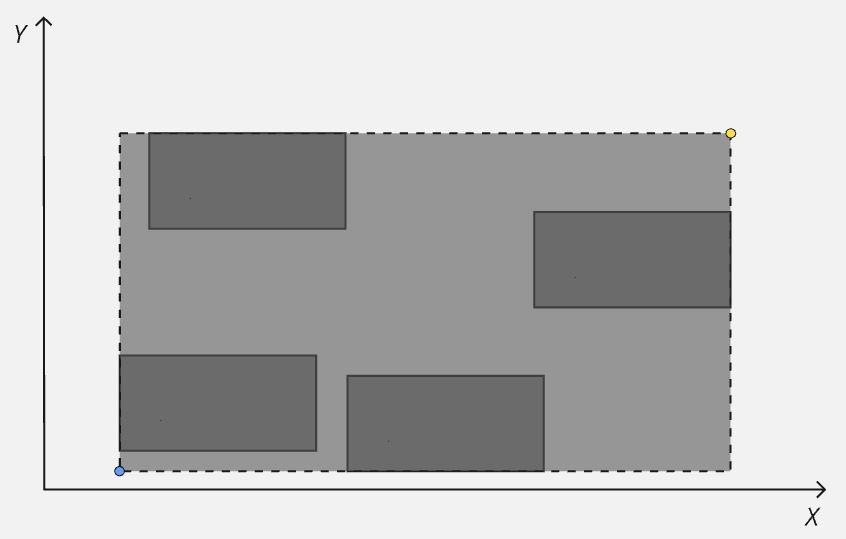
\includegraphics[width=0.6\textwidth]{figures/Orden/image.png}
  \caption{Representación gráfica del conjunto dominio de un mapa con 4 multi-intervalos, más el marcado del mínimo y máximo perimetral en azul y amarillo respectivamente.}
  \label{fig:minmaxPer1}
\end{figure}


Con toda esta información ya se puede declarar formalmente cómo está constituida la variable \texttt{pieces\_} para los \textit{piecewise maps} ordenados, denominados como \texttt{OrdPWMap}:

\begin{itemize}
  \item \texttt{pieces\_} (de tipo \textbf{OrdMapCollection}): 
  representa la colección ordenada de mapas junto con la información perimetral 
  de sus dominios.  
  En este contexto:
  \begin{itemize}
    \item \texttt{OrdMapCollection} es sinónimo de \texttt{vector<MapEntry>}.
    \item \texttt{MapEntry}, cuyas instancias denominaremos en adelante \textit{entradas de mapa}, es sinónimo de \texttt{pair<Map, SetPerimeter>}.
    \item \texttt{SetPerimeter}, cuyas instancias denominaremos en adelante \textit{perímetros}, es sinónimo de \texttt{pair<MD\_NAT, MD\_NAT>}.
  \end{itemize}
\end{itemize}


Y por último se presenta el siguiente ejemplo. Sean se los siguientes conjuntos dominio de los mapas $m_1$, $m_2$, y $m_3$ respectivamente:

\begin{itemize}
    \item $c_1 = \{[10:1:15]\times[10:1:11],[16:1:20]\times[15:1:20]\}$, con mínimo perimetral $(10,10)$
    \item $c_2 = \{[15:1:20]\times[15:1:25],[21:1:25]\times[15:1:20]\}$, con mínimo perimetral $(15,15)$
    \item $c_3 = \{[30:1:35]\times[15:1:20],[36:1:40]\times[10:1:11]\}$, con mínimo perimetral $(30,10)$
\end{itemize}

Aplicando el criterio de orden basado en los mínimos perimetrales, junto con el operador $<$ definido para la naturales multi-dimensionales, se obtiene el siguiente ordenamiento:

\begin{center}
\[
c_1 < c_2 < c_3
\]

ya que:

\[
(10,10) < (15, 15) < (30, 10)
\]

Por lo tanto, el conjunto ordenado resultante será:

\[
\ll (m_1,(minPer_1, maxPer1)),\ (m_2,(minPer_2, maxPer2)),\ (m_3, (minPer_3, maxPer3))\gg
\]
\end{center}

\section{\textit{Abstarct factory}}

Al igual que se hizo con los \textit{piecewise maps} desordenados,
también se definió la fábrica concreta para los \textit{Piecewise maps} ordenados, para poder aplicar el patrón \textit{Abstarct factory}. 

En particular, la fábrica concreta de los \textit{Piecewise maps} ordenados se denominó 
\texttt{PWMapAF}. Esta puede encontrarse en los archivos 
\textit{af\_pwmap}, tanto en su versión 
\textit{.cpp} como \textit{.hpp}, dentro de la carpeta \texttt{sbg} del repositorio.

\section{Criterios de optimización y ordenamiento}\label{sec:pwmap-opts}

En esta sección se describen en detalle los distintos \textbf{criterios de optimización} y \textbf{ordenamiento} utilizados en las operaciones sobre \textit{piecewise maps} ordenados. Ambos conjuntos de criterios serán aplicados con el propósito de mejorar la eficiencia general de dichas operaciones y reducir significativamente los tiempos de ejecución.

\textbf{Pseudocódigo y notación:} En esta sección, al igual que se hizo para los \textit{piecewise maps} desordenados, se emplearán subíndices para referirse a los mapas de un \textit{piecewise map} ordenado con el fin de aliviar la notación. Dado un \textit{piecewise map} ordenado $A$, el elemento ubicado en la posición $i$, lo cual corresponde a \texttt{pieces\_[i].first} en C++, se denotará como \textbf{$A_i$}, donde $i$ es un número natural que satisface $0 \leq i < \kappa(A)$, siendo $\kappa(A)$ la cantidad de mapas de $A$. Cabe destacar que, al tratarse de un \textit{piecewise map} ordenado, siempre se cumple que $A_i < A_j$ si y sólo si $i < j$, para todo par de $i$ y $j$ tal que $0  \leq i, j < \kappa(A)$. Adicionalmente se dirá que, en el caso anterior, $A_i$ está \textbf{antes} de $A_j$ en $A$, mientras $A_j$ está \textbf{después} de $A_i$.

\subsection{Operaciones estructuralmente similares}

Como se puede ver en la Sub-sección \ref{sec:pwmaps-des} existen muchas operaciones que presentan una estructura muy similar a la de la intersección entre conjuntos desordenados. Entre estas operaciones se encuentran: la \textbf{igualdad}, la \textbf{suma}, la i\textbf{gualdad de imágenes}, la \textbf{resta} y el \textbf{mínimo adyacente}.

Todas estas operaciones, junto con la intersección de conjuntos ordenados, comparten una estructura común que se puede dividir en dos partes: 
\begin{enumerate}
    \item Una\textbf{ fase de comparación}, donde cada elemento de uno de los argumentos es comparado con todos los del otro argumento.
    \item Un \textbf{núcleo de la operación}, donde se ejecuta la lógica específica de la operación sobre aquellos pares de elementos cuya comparación fue satisfactoria.
\end{enumerate}

Esta estructura puede observarse gráficamente en el pseudocódigo presentado en ~\ref{alg:operaciones-simil}.

En el caso de la intersección de conjuntos desordenados, la comparación consiste en verificar si la intersección entre dos multi-intervalos, uno de cada conjunto, es vacía, y el núcleo de la operación se encarga de guardar dicha intersección en el conjunto resultante.

En cambio, para las otras operaciones mencionadas, la comparación consiste en verificar si la intersección entre los dominios de dos mapas, uno de cada \textit{piecewise map} desordenado argumento, es no vacía. El núcleo depende de la operación específica: por ejemplo, en el caso de la suma, se calcula la suma de los mapas y se almacena el resultado en el \textit{piecewise map} desordenado de salida.


\begin{algorithm}
\caption{Estructura de las operaciones similares a la intersección de conjuntos desordenados}\label{alg:operaciones-simil}
\begin{algorithmic}[1]
\Require $A$, $B$ son conjuntos desordenados o dos \textit{piecewise maps} desordenados
\Function{operación}{$A, B$}

\State ... \Comment{Casos base y definiciones necesarias de la operación}

\ForAll{$a \in A$} \Comment{Fase de comparación de la operación.}
    \ForAll{$b \in B$}
        \State $I$ \Comment{Elemento a comparar proveniente de una o varias operaciones entre los elementos $a$ y $b$}
        \If{$\Call{isEmpty}{I}$}
            \State ...  \Comment{Núcleo de la operación.}
        \EndIf
    \EndFor
\EndFor

\State \Return ...
\EndFunction
\end{algorithmic}
\end{algorithm}

Por lo tanto, dado que las operaciones sobre \textit{piecewise maps} desordenados mencionadas anteriormente comparten esta misma estructura, y considerando todas las definiciones introducidas para los \textit{piecewise maps} ordenados, es posible adaptar los criterios de optimización desarrollados para la intersección de conjuntos ordenados a las operaciones mencionadas de  \textit{piecewise maps} ordenados.

\subsubsection{Criterios de optimización}

\begin{center}
    \fbox{
        \parbox{0.92\linewidth}{
            \centering
            \textbf{Criterio de parada} \\[1ex]
            \raggedright
            Sean $A$ y $B$ dos \textit{piecewise maps} ordenados. Supóngase que se está evaluando una de las operaciones mencionadas entre ambos, y en particular se consideran los posibles cálculos del núcleo de la operación entre mapa $A_i$ de $A$, con $0 \leq i < \kappa(A)$, y los mapas de $B$. Dado un índice $j$ tal que $0 \leq j < \kappa(B)$, vale lo siguiente:

            \vspace{0,5cm}
     
            \textbf{Si} el máximo perimetral del dominio de $A_i$ es estrictamente menor que el mínimo perimetral del dominio de $B_j$ en la primera dimensión, \textbf{entonces}:

            \begin{itemize}
                \item la intersección entre el dominio de $A_i$ y el de $B_{j'}$ resulta vacía \textbf{y} no se calcula el núcleo de la operación para $A_i$ y $B_{j'}$, $\forall j' \mid j \leq j' < |B|$;
                \item \textbf{y, entonces,} puede continuarse directamente con la fase de comparación entre $A_{i+1}$(si existe) y los mapas de $B$ para validar el calculo del núcleo de la operación.
            \end{itemize}
    
        }
    }
\end{center}



\begin{center}
    \fbox{
        \parbox{0.92\linewidth}{
            \centering
            \textbf{Criterio de eliminación} \\[1ex]
            \raggedright
            Sean $A$ y $B$ dos \textit{piecewise maps} ordenados. Supóngase que se está evaluando una de las operaciones mencionadas entre ambos, y en particular se consideran los posibles cálculos del núcleo de la operación entre mapa $A_i$ de $A$, con $0 \leq i < \kappa(A)$, y los mapas de $B$. Dado un índice $j$ tal que $0 \leq j < \kappa(B)$, vale lo siguiente:

            \vspace{0,5cm}
     
            \textbf{Si} el máximo perimetral del dominio de $(B_{j}$ es estrictamente menor que al mínimo perimetral del conjunto $A_{i}$ en la primera dimensión, \textbf{entonces}:

            \begin{itemize}
                \item la intersección entre $A_{i'}$ y $B_{j}$ resulta vacía \textbf{y} no se calcula el núcleo de la operación para $A_{i'}$ y $B_{j}$, $\forall i' \mid i \leq i' < \kappa(A)$;
                
                \item \textbf{y, entonces,} puede descartarse $B_j$ para las fases de comparación de los mapas posteriores a $A_i$ y así descartar completamente el calculo del núcleo de la operación $B_j$ con estos.
            \end{itemize}
                
    
        }
    }
\end{center}



\begin{center}
    \fbox{
        \parbox{0.9\linewidth}{
            \centering
            \textbf{Criterio de selección} \\[1ex]
            \raggedright
            Sean dos piecewise maps ordenados involucrados en alguna de las operaciones mencionadas. Se establece lo siguiente:

            \begin{center}
            \textit{
                Se define como $B$ a aquel piecewise map que contiene la menor cantidad de mapas,
                mientras que se denota como $A$ al piecewise map restante.
            }
            \end{center}
        }
    }
\end{center}


\begin{center}
    \fbox{
        \parbox{0.93\linewidth}{
            \centering
            \textbf{Criterio de solapamiento} \\[1ex]
            \raggedright
            Sean $A$ y $B$ dos \textit{piecewise maps}, $A_i$ un mapa de $A$ y $B_j$ uno de $B$, con índices tales que:
            \[
            0 \leq i < \kappa(A), \quad 0 \leq j < \kappa(B).
            \]
            Se establece entonces que, en el caso de realizar una de las operaciones entre $A$ y $B$, y querer calcular el núcleo de la operación entre $A_i$ y 
            $B_j$:

            \begin{itemize}
                \item \textbf{Si} existe solapamiento entre los conjuntos dominio de $A_i$ y $B_j$, \textbf{entonces}:
                \begin{itemize}
                    \item \textbf{Si} ambos conjuntos son \textit{densos}, la intersección entre ellos es necesariamente no vacía y se puede proceder con el calculo del núcleo de la operación.
                    \item \textbf{Si} al menos uno de ellos no es denso, la intersección \textit{puede} ser no vacía, pero no se garantiza de modo que se debe proceder de igual manera.
                \end{itemize}

                \item \textbf{Si} \textbf{no} existe solapamiento entre los conjuntos dominio de $A_i$ y $B_j$, \textbf{entonces} la intersección entre ellos es necesariamente vacía, independientemente de si son densos o no, y por ende puede obviarse el calculo del núcleo de la operación.
            \end{itemize}
        }
    }
\end{center}


En este último caso faltaría definir qué es el solapamiento entre conjuntos y cuándo un conjunto es denso para poder completar el criterio anterior:

        \begin{center}
            Sean $C$ y $D$ dos conjuntos. Entonces se dice que $C$ y $D$ se solapan o están solapados si y solo si los multi-intervalos definidos a través de sus mínimos y máximos perimetrales se solapan bajo la definición de solapamiento de multi-intervalos ya vista.
        \end{center}

        \begin{figure}[h]
    \centering
    \begin{subfigure}[b]{0.48\linewidth}
        \centering
        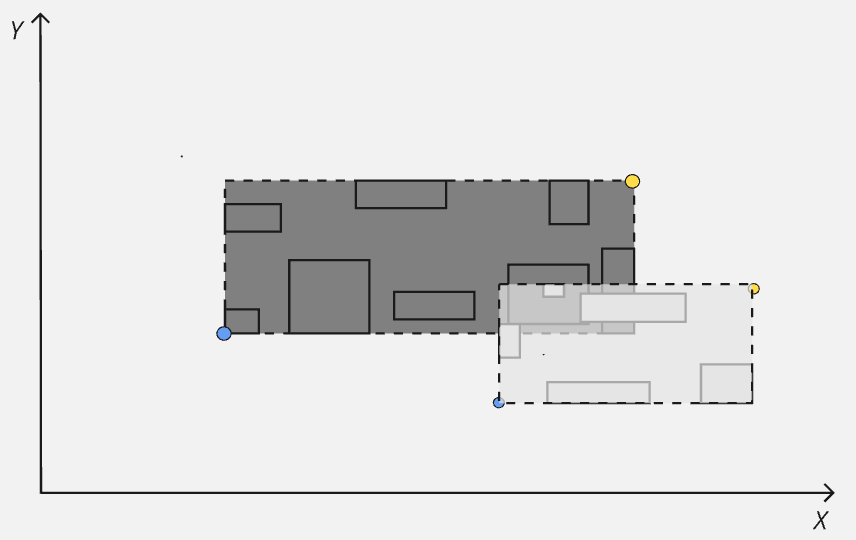
\includegraphics[width=\linewidth]{figures/optimizaciones pwmap/op simils/mi1.png}
        \caption{Conjuntos con sus multi-intervalos definidos con sus máximos y mínimos perimetrales.}
        \label{fig:crit-suma-dominio}
    \end{subfigure}
    \hfill
    \begin{subfigure}[b]{0.48\linewidth}
        \centering
        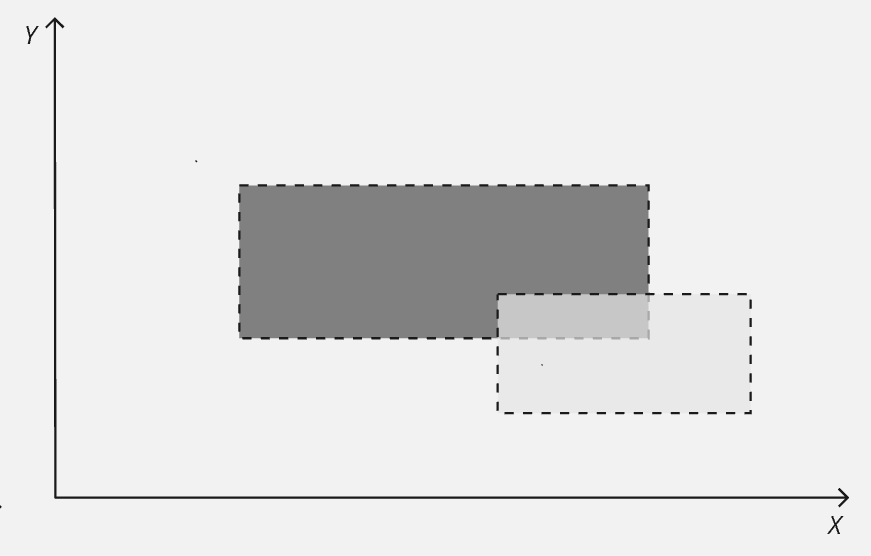
\includegraphics[width=\linewidth]{figures/optimizaciones pwmap/op simils/mi2.png}
        \caption{Solapamiento entre los multi-intervalos definidos.}
        \label{fig:crit-suma-extremos}
    \end{subfigure}
    \caption{Criterios de solapamiento para \textit{piecewise maps} ordenados.}
    \label{fig:crit-suma}
\end{figure}

        \begin{center}
            Sea $C$ el conjunto, y sean $minPer_C$ y $maxPer_C$ el mínimo y máximo perimetral, respectivamente. Entonces se dice que el conjunto es \textbf{denso} si y solo si, si se define un multi-intervalo denso $mdi$ donde su mínimo y máximo sean $minPer_C$ y $maxPer_C$ respectivamente, entonces:
                \[
                    \{mdi\} - C = C - \{mdi\} = \emptyset
                \]
        \end{center}
\begin{figure}[h]
    \centering
    \begin{subfigure}[b]{0.42\linewidth}
        \centering
        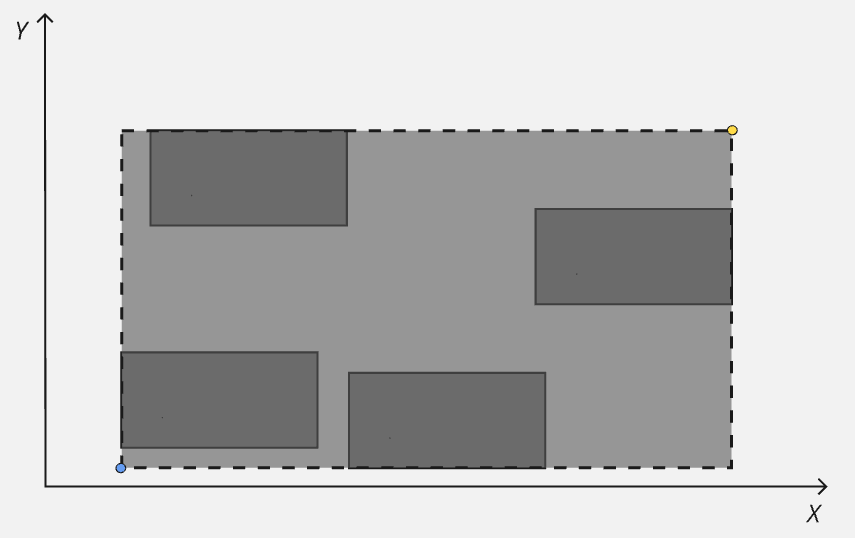
\includegraphics[width=\linewidth]{figures/optimizaciones pwmap/op simils/denso1.png}
        \caption{Conjunto no denso.}
        \label{fig:crit-suma-dominio}
    \end{subfigure}
    \hfill
    \begin{subfigure}[b]{0.42\linewidth}
        \centering
        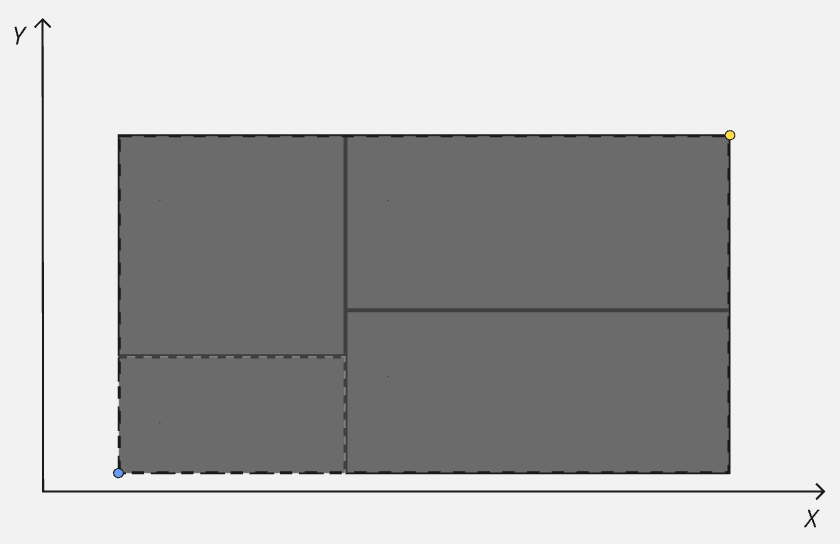
\includegraphics[width=\linewidth]{figures/optimizaciones pwmap/op simils/denso2.png}
        \caption{Conjunto no denso.}
        \label{fig:crit-suma-max}
    \end{subfigure}
    \hfill
    \vspace{0,5cm}
    \begin{subfigure}[b]{0.42\linewidth}
        \centering
        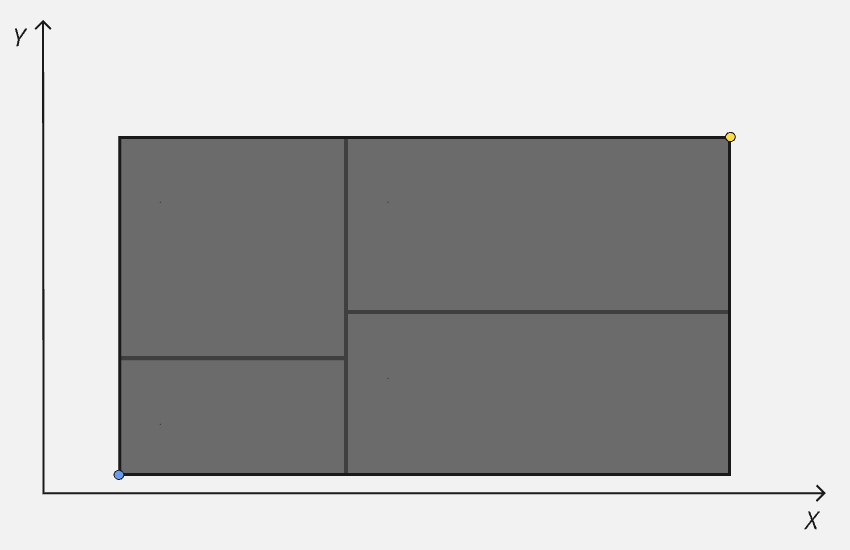
\includegraphics[width=\linewidth]{figures/optimizaciones pwmap/op simils/denso3.png}
        \caption{Conjunto denso.}
        \label{fig:crit-suma-min}
    \end{subfigure}
    \caption{Densidad de conjuntos.}
    \label{fig:crit-suma}
\end{figure}





\subsubsection{Criterios validos por operación}

Ahora bien, el núcleo de la operación puede variar significativamente dependiendo de la naturaleza de la operación considerada. En consecuencia, el criterio de ordenamiento utilizado también puede diferir considerablemente entre una operación y otra. 

Por esta razón, los criterios específicos serán mencionados y analizados individualmente, operación por operación. 

Además, no todas las operaciones admitirán todos los criterios de optimización previamente definidos. La aplicabilidad de cada criterio dependerá de las particularidades del núcleo de la operación y del comportamiento esperado.


\textbf{Igualdad - \texttt{==}}

Para el caso de la igualdad, se pueden aplicar todos los criterios de optimización previamente definidos. 

En cuanto a su \textbf{criterio de ordenamiento}, esta operación no requiere de uno, ya que no produce como resultado un \textit{piecewise map} ordenado. En consecuencia, no dispone de un criterio de ordenamiento asociado.

\textbf{suma - \texttt{+}}

En el caso de la suma, vuelven a aplicarse todos los criterios de optimización mencionados. Y, en cuanto a su criterio de ordenamiento, este resulta muy similar al propuesto para la intersección de conjuntos ordenados, con las modificaciones y adaptaciones necesarias claro esta.


\begin{center}
    \fbox{
        \parbox{0.93\linewidth}{
            \centering
            \textbf{Criterio de ordenamiento} \\[1ex]
            \raggedright
            Supóngase que se realiza la suma entre dos \textit{piecewise maps} ordenados, $A$ y $B$, y que se están evaluando las posibles sumas del $i$-ésimo mapa de $A$, denotado por $A_i$, con todos los mapas de $B$. Ademas se cuenta con un \textit{piecewise map} resultado $C$.

            \vspace{1ex}

            Todas las sumas no vacías generadas con $A_i$ deben insertarse en $C$ \textbf{después} de aquellas sumas generadas por los mapas $A_0, A_1, \dots, A_{i-1}$, cuyos mínimos perimetrales sean estrictamente menores al mínimo perimetral de $A_i$, bajo el operador $<$ de naturales multi-dimensionales.
        }
    }
\end{center}

Este criterio se basa nuevamente en la observación de que, al realizar la \textit{suma}, 
su dominio corresponde a la intersección de los dominios de los mapas participantes. 
Dicha intersección entre dos dominios está contenida en ambos, lo que implica que su mínimo perimetral 
se encuentra dentro de los multi-intervalos definidos por el mínimo y el máximo perimetral de los operandos.  

Al fijar \(A_i\), todas sus sumas posibles con mapas de \(B\) tendrán su mínimo perimetral dentro del multi-intervalo definido por el mínimo y el máximo perimetral de \(A_i\). 
Como consecuencia, cualquier suma con dominio no vacío generada tendrá un mínimo perimetral mayor o igual 
que el mínimo perimetral de \(A_i\), bajo el operador $<$ de los naturales multi-dimensionales.


Esto garantiza que tales sumas deben insertarse en el \textit{piecewise map} resultado después de aquellas cuyo 
 dominio tenga un mínimo perimetral que sea estrictamente menor,bajo el operador $<$ de los naturales multi-dimensionales, al de $A_i$, es decir, las generadas por los mapas anteriores de $A$. Una vez procesado $A_i$, se avanza hacia $A_{i+1}$ y se continúa la construcción del \textit{piecewise map} resultado de la misma manera.

La Figura~\ref{fig:crit-suma} ilustra gráficamente esta situación. Allí se observa todas las intersecciones de los dominios de las sumas producidas a partir del mapa $A_i$ con los mapas de $B$. En particular los dominios tienen el mismo nombre que los mapas a los que pertenecen. Y como se ve, estas sumas que realizan la intersección de sus dominios tienen un mínimo perimetral mayor o igual que el del dominio de $A_i$, y se insertan a continuación de los mapas previamente procesadas cuyo mínimo perimetral sea menor al de $A_i$. Esto mismo ocurre con las de $A_{i+1}$ cuya suma con $B_k$ se debe insertar después de los mapas con $A1$ y  $A2$ como dominio.

\begin{figure}[h]
    \centering
    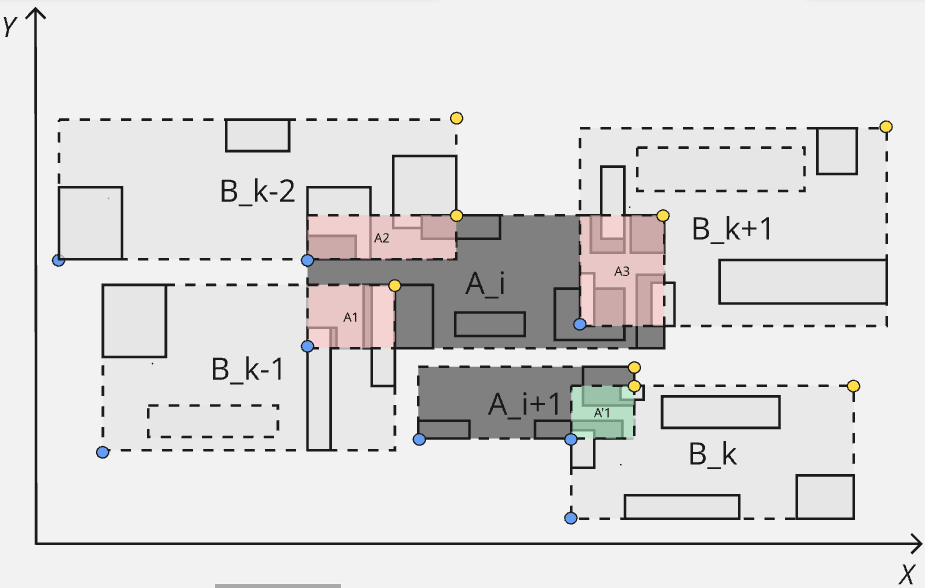
\includegraphics[width=0.8\linewidth]{figures/optimizaciones pwmap/op simils/crit suma.png}
    \caption{Criterio de ordenamiento de la suma para \textit{piecewise map} ordenados de las sumas en función de su dominio y, en particular, de sus mínimos perimetrales.}
    \label{fig:crit-suma}
\end{figure}

Adicionalmente, no es necesario comenzar a verificar la posición de inserción de las sumas en el \textit{piecewise map} resultado desde el principio en cada iteración de los elementos de $A$. Dado el orden intrínseco de los \textit{piecewise map} involucrados, se cumple que
\[
minPer_{i} \leq minPer_{i+1}
\]
 donde $minPer_i$ y $minPer_{i+1}$ son los minimos perimetrales de $A_i$ y $A_{i+1}$ respectivamente.
 
Esto implica que las sumas generadas por $A_{i+1}$ necesariamente deben insertarse a partir de una posición igual o posterior a aquella donde comenzaron a colocarse las sumas de $A_i$ con los elementos de $B$.

Esto desencadena la siguiente modificación del criterio de ordenamiento: 
\begin{center}
    \fbox{
        \parbox{0.93\linewidth}{
            \centering
            \textbf{Criterio de ordenamiento} \\[1ex]
            \raggedright
            Supóngase que se realiza la suma entre dos \textit{piecewise maps} ordenados, $A$ y $B$, y que se están evaluando las posibles sumas del $i$-ésimo mapa de $A$, denotado por $A_i$, con todos los mapas de $B$. Ademas se cuenta con un \textit{piecewise map} resultado $C$.

            \vspace{1ex}

            Todas las sumas no vacías generadas con $A_i$ deben insertarse en $C$ \textbf{después} de aquellas sumas generadas por los mapas $A_0, A_1, \dots, A_{i-1}$, cuyos mínimos perimetrales sean estrictamente menores al mínimo perimetral $A_i$, bajo el operador $<$ de naturales multi-dimensionales.
            
            \vspace{1ex}

            Adicionalmente \textbf{si} la posición a partir de la cual se colocan las sumas de $A_i$ en el \textit{piecewise map} resultante es $j$, con $0 \leq j < \kappa(C)$, \textbf{entonces} aquellas generadas por $A_{i+1}$ se insertaran a partir de $j'$ tal que $j \leq j' < \kappa(C)$.
        }
    }
\end{center}

\textbf{Igualdad de imágenes - \texttt{equalImage}}

El caso de esta operación es muy similar al de la operación de igualdad: admite todos los criterios de optimización y tampoco requiere un criterio de ordenamiento. Esta última característica, a diferencia del caso de la igualdad, no se debe a que la operación devuelva un valor de verdad, sino a que su resultado es un conjunto en sí mismo, el cual tiene su implementación propia y no se debe alterar.


\textbf{Mínimo adyacente - \texttt{minAdjMap}}

Ahora es el turno de la operación \texttt{minAdjMap}, la cual puede utilizar todos los criterios de optimización, salvo el de selección, ya que nuevamente el orden de los argumentos tiene relevancia. 

En cuanto al criterio de ordenamiento, aparece un problema que se repite tanto aquí como en varias operaciones sobre \textit{piecewise maps} ordenados: la imagen. La imagen de un mapa, aunque es un conjunto, posee una cohesión que depende tanto del conjunto dominio como de la colección de expresiones lineales del mapa. Por ejemplo, dos mapas pueden tener un mismo dominio, pero basta con que alguna de sus expresiones varíe para que sus imágenes sean distintas. Algo similar ocurre si varía el dominio.

Entonces, ordenar mapas cuyo dominio corresponde a la imagen resulta una tarea particularmente compleja. En estos casos, el orden del \textit{piecewise map} original aporta escasa o nula información útil para ordenar los mapas derivados, cuyos dominios provienen de una imagen. 

Una alternativa es realizar un ordenamiento estrictamente lineal, lo cual implica un costo computacional elevado, especialmente cuando el \textit{piecewise map} resultante contiene un gran número de mapas.


En conclusión, para poder brindar un orden a un \textit{piecewise map} cuyo contenido son mapas con dominios derivados de imágenes, sería necesario tener en cuenta no solo el dominio, sino también las expresiones y la forma de dichas expresiones. Por esta razón, se concluyó que lo más óptimo es utilizar un algoritmo de ordenamiento preexistente, lo cual simplifica el entendimiento de esta y de las demás operaciones de \textit{piecewise maps} ordenados. Así se evita la necesidad de escribir y mantener código de criterios de ordenamiento que, probablemente, tendría un rendimiento inferior.


\textbf{Resta - \texttt{-}}

Por ultimo se encuentra la operación \texttt{-}, la cual admite todos los criterios de optimización, con excepción del criterio de selección, ya que se trata de una operación donde el orden de los argumentos es relevante y, por lo tanto, no puede alterarse. En cuanto al orden de la salida, ocurre algo particular. 

En el núcleo de la operación desordenada, cuando se calcula la resta entre dos mapas, el proceso genera un resultado parcial únicamente para los dos mapas involucrados. El tamaño de este resultado parcial, o la cantidad de mapas que contiene, depende exclusivamente de la cantidad de dimensiones con las que se esté trabajando. Luego, este resultado parcial se incorpora al \textit{piecewise map} resultado de la operación.

Ahora bien, para garantizar que la salida se encuentre correctamente ordenada, se optó por emplear un algoritmo de ordenamiento preexistente. De este modo, se evita mantener la invariante de orden durante la operación en el \textit{piecewise map} resultante y en el resultado parcial, y en su lugar, antes de devolver el \textit{piecewise map} resultante, se procede a ordenarlo utilizando dicho algoritmo.

De esta forma, se evita recurrir a estrategias ineficientes, como ordenar cada resultado parcial para luego aplicar la operación \texttt{concatenation}.

\subsection{Restricción de dominio - \texttt{restrict}}

El caso de la operación \texttt{restrict} es diferente al de las operaciones vistas anteriormente. Sin embargo, esto no significa que no puedan adaptarse los criterios definidos previamente para esta operación.

En particular, la operación \texttt{restrict} aplicada a un \textit{piecewise map} desordenado, como ya se vio, consiste en restringir el dominio de cada uno de sus mapas individuales en base a un conjunto, siendo ambos argumentos de la operación, y quedando como parte del resultado solo aquellos mapas del \textit{piecewise map} desordenado cuyos dominios restringidos son no vacíos.

Ahora bien, al dotar de orden al \textit{piecewise map} argumento y requerir que el resultado también esté ordenado, la operación puede beneficiarse de los siguientes criterios de optimización y ordenamiento:

\subsubsection{Criterios de optimización}


\begin{center}
    \fbox{
        \parbox{0.92\linewidth}{
            \centering
            \textbf{Criterio de parada} \\[1ex]
            \raggedright
            Sean $A$ un \textit{piecewise map} ordenado y $S$ un conjunto. Supóngase que se evalúa la restricción de dominio entre ambos, y en particular se considera la posible restricción de domino del dominio de un mapa $A_i$ de $A$, con $0 \leq i < \kappa(A)$, con respecto a $S$. Entonces vale lo siguiente:

            \vspace{0,5cm}
     
            \textbf{Si} el máximo perimetral de $S$ es estrictamente menor que el mínimo perimetral del conjunto dominio de $A_i$ en la primera dimensión, \textbf{entonces}:

            \begin{itemize}
                \item la intersección entre el dominio de $A_i$ y $S$ resulta vacía \textbf{y} no se calcula la restricción de dominio para $A_{i'}$ con respecto a $S$, $\forall i' \mid i \leq i' < \kappa(A)$;
                \item \textbf{y, entonces,} puede terminarse directamente con la operación \texttt{restrict}.
            \end{itemize}
    
        }
    }
\end{center}


\begin{center}
    \fbox{
        \parbox{0.93\linewidth}{
            \centering
            \textbf{Criterio de solapamiento} \\[1ex]
            \raggedright
            Sean $A$ un \textit{piecewise map}, $S$ un conjunto y $A_i$ un mapa de $A$ tal que:
            \[
            0 \leq i < \kappa(A).
            \]
            Se establece entonces que, en el caso de realizar la restricción de dominio de $A$ sobre $S$ y querer calcular la restricción de $A_i$ con respecto a $S$:

            \begin{itemize}
                \item \textbf{Si} existe solapamiento entre el conjunto dominio de $A_i$ y $S$, \textbf{entonces}:
                \begin{itemize}
                    \item \textbf{Si} ambos conjuntos son \textit{densos}, la intersección entre ellos es necesariamente no vacía y se puede proceder con el calculo de la restricción del dominio de $A_i$ en base a $S$.
                    \item \textbf{Si} al menos uno de ellos no es denso, la intersección \textit{puede} ser no vacía, pero no se garantiza de modo que se debe proceder de igual manera.
                \end{itemize}

                \item \textbf{Si} \textbf{no} existe solapamiento entre el conjunto dominio de $A_i$ y $S$, \textbf{entonces} la intersección entre ellos es necesariamente vacía, independientemente de si son densos o no, y por ende puede obviarse el calculo de la restricción del dominio de $A_i$ en base a $S$.
            \end{itemize}
        }
    }
\end{center}

\subsubsection{Criterio de ordenamiento}

En este caso, lo que debe mantenerse ordenado en el \textit{piecewise map} resultante son todas las restricciones de dominio no vacías de los mapas del \textit{piecewise map} ordenado argumento. La restricción de dominio de un mapa consiste únicamente en reemplazar su dominio original por la intersección entre dicho dominio y el conjunto que también llega como argumento.

Ahora bien, como se discutió en el criterio de ordenamiento para la suma, el mínimo perimetral del dominio restringido está contenido dentro de alguno de los multi-intervalos definidos por los máximos y mínimos perimetrales del dominio del mapa a restringir y del conjunto que restringe. Ademas aquí también vale que no es necesario buscar la posición de inserción desde el comienzo del \textit{piecewise map} resultado. Esto permite redefinir el criterio de ordenamiento de la siguiente manera:

\begin{center}
    \fbox{
        \parbox{0.93\linewidth}{
            \centering
            \textbf{Criterio de ordenamiento} \\[1ex]
            \raggedright
            Supóngase que se realiza la restricon de dominio entre un \textit{piecewise map} ordenado $A$ y un conjunto $S$, y que se están evaluando la restricción de dominio del $i$-ésimo mapa de $A$, denotado por $A_i$, con respecto a $S$. Ademas se cuenta con un \textit{piecewise map} resultado $C$.

            \vspace{1ex}

            La restricción no vacía generada con $A_i$ deben insertarse en $C$ \textbf{después} de aquellas restricciones no vacías generadas por los mapas $A_0, A_1, \dots, A_{i-1}$, cuyos mínimos perimetrales sean estrictamente menores al mínimo perimetral de $A_i$, bajo el operador $<$ de naturales multi-dimensionales.

            \vspace{1ex}

            Adicionalmente \textbf{si} la posición a partir de la cual se colocan las sumas de $A_i$ en el \textit{piecewise map} resultante es $j$, con $0 \leq j < \kappa(C)$, \textbf{entonces} aquellas generadas por $A_{i+1}$ se insertaran a partir de $j'$ tal que $j \leq j' < \kappa(C)$.
        }
    }
\end{center}


\subsection{Combinación - \texttt{combine}}

El siguiente caso que se analizará es el de la operación \texttt{combine}, una de las ya introducidas previamente en el capítulo de conceptos preliminares.

Esta operación, como ya se vio, aplicada sobre \textit{piecewise maps} desordenados, toma dos de ellos y realiza una suerte de unión, devolviendo un único \textit{piecewise map} desordenado. Este contiene todos los mapas del primero, junto con aquellos mapas del segundo cuyos dominios son una restricción, conteniendo ahora solo aquellos valores no presentes en el dominio total del primer \textit{piecewise map}. 

Debido a la naturaleza de su funcionamiento y requerir preservar el orden en el resultado, esta operación emplea únicamente un criterio de optimización y un criterio de ordenamiento, ambos reformulados de los vistos para las \textit{operaciones estructuralmente similares}.

\subsubsection{Criterio de optimización}

Trabajando con dos \textit{piecewise maps} $A$ y $B$, los únicos mapas de $B$ que pueden formar parte del resultado son aquellos donde la diferencia de su domino con el dominio total de $A$ sea no vacía. El dominio modificado resultante para cada uno de los mapas de $B$ será precisamente dicha diferencia. Por lo tanto, lo único que se puede hacer es omitir la diferencia cuando se sabe que no es necesaria, y de esta observación se deriva el siguiente criterio de solapamiento:

\begin{center}
    \fbox{
        \parbox{0.93\linewidth}{
            \centering
            \textbf{Criterio de solapamiento} \\[1ex]
            \raggedright
            Sean $A$ y $B$ dos \textit{piecewise maps}, $B_j$ un mapa de $B$, tal que:
            \[
            0 \leq j < \kappa(B).
            \]
            y sea $S$ el dominio de $A$. Se establece entonces que, en el caso de realizar la combinación entre $A$ y $B$ y al estar considerando $B_j$ :

            \begin{itemize}
                \item \textbf{Si} existe solapamiento entre el conjunto dominio de $B_j$ y $S$, \textbf{entonces}:
                \begin{itemize}
                    \item \textbf{Si} ambos conjuntos son \textit{densos}, la intersección entre ellos es necesariamente no vacía y se debe proceder con el calculo de la diferencia para obtener el nuevo dominio de $B_j$.
                    \item \textbf{Si} al menos uno de ellos no es denso, la intersección \textit{puede} ser no vacía, pero no se garantiza de modo que se debe proceder de igual manera.
                \end{itemize}

                \item \textbf{Si} \textbf{no} existe solapamiento entre el conjunto dominio de $B_j$ y $S$, \textbf{entonces} la intersección entre ellos es necesariamente vacía, independientemente de si son densos o no, y por ende puede obviarse el calculo de la diferencia,la cual devolvería el mismo dominio de $B_j$, y el dominio de $B_k$ queda intacto.
            \end{itemize}
        }
    }
\end{center}

\subsubsection{Criterio de ordenamiento}

En cuanto al orden, al realizar la diferencia entre dos conjuntos, por ejemplo, entre dos conjuntos $C$ y $D$, el nuevo mínimo perimetral del conjunto resultante $C - D$ debe encontrarse contenido dentro del multi-intervalo definido por el mínimo y el máximo perimetral del conjunto original $C$. 

Esto se debe a que la operación de diferencia remueve elementos de $C$, sin añadir otros nuevos. Esta observación es casi análoga a lo que ocurría en el caso de la operación de suma, discutido en en este capitulo con respecto a la suma de \textit{piecewise map} ordenados. Análogamente a lo visto también en la suma, gracias a lo anterior y al orden de los \textit{piecewise maps}, ocurre que si $B_j$ con su dominio modificado se debería insertar a partir de una posición $i$, con $0 \leq i < \kappa(C)$, en el \textit{piecewise map} resultado, entonces $B_j$ con su dominio modificado debería ubicarse en $i'$ tal que $i \leq i' < \kappa(C)$

En consecuencia, se postula el siguiente criterio de ordenamiento derivado del visto para el operador \texttt{+}:

\begin{center}
    \fbox{
        \parbox{0.93\linewidth}{
            \centering
            \textbf{Criterio de ordenamiento} \\[1ex]
            \raggedright
            Supóngase que se realiza la combinación entre dos \textit{piecewise maps} ordenados, $A$ y $B$, y que se deba calcular el nuevo dominio para el mapa $j$-ésimo de $B$, denotado por $B_j$, con respecto al dominio de $A$, $S$. Ademas se cuenta con un \textit{piecewise map} resultado $C$.

            \vspace{1ex}

            \textbf{Si} el nuevo dominio de $B_j$ no es vacío, es decir, la resta entre el conjunto dominio de $B_j$ y $S$ es no vacía; \textbf{entonces} el mapa $B_j$ con dominio restringido por $S$ estará ubicado en el \textit{piecewise map} resultante después de todos aquellos mapas cuyo mínimo perimetral sea menor que el minino perimetral del dominio original de $B_j$, bajo el operador $<$ de naturales multi-dimensionales.
            
            \vspace{1ex}

            Adicionalmente \textbf{si} la posición a partir de la cual se coloca de $B_j$ con dominio modificado en el \textit{piecewise map} resultante es $i$, con $0 \leq i < \kappa(C)$, \textbf{entonces} el mapa modificado de $B_{j+1}$ se insertaría, si su dominio no es vacío, a partir de $i'$ tal que $i \leq i' < \kappa(C)$.
        }
    }
\end{center}


\subsection{Concatenación - \texttt{concatenation}}

El caso de la operación concatenación, es básicamente homólogo al del la unión disjunta de conjuntos, y por ende haciendo las respectivas modificaciones, se puede reutilizar lo visto para la unión disjunta de conjuntos ordenados aquí.

\subsubsection{Criterio de ordenamiento}

\begin{center}
    \fbox{
        \parbox{0.93\linewidth}{
            \centering
            \textbf{Criterio de ordenamiento}\\[1ex]
            \raggedright
           Sean $A = \{A_0, A_1, \dots, A_{n-1}\}$ y $B = \{B_0, B_1, \dots, B_{m-1}\}$ dos \textit{piecewise maps} no vacíos, disjuntos y ordenados. Sea $C$ un \textit{piecewise map} inicialmente vacío que contendrá el resultado de la fusión ordenada de $A$ y $B$. Y sean $A_i$ un mapa de $A$ y $B_j$ un mapa de $B$, con índices tales que:
            \[
            0 \leq i < \kappa(A), \quad 0 \leq j < \kappa(B).
            \]
            
            \vspace{1ex}

            Entonces, al realizar la unión disjunta entre $A$ y $B$ vale que:

            \begin{itemize}
                \item \textbf{Si} el mínimo perimetral de  $A_i$ es menor, bajo el operador $<$ definido para naturales multi-dimensionales, que el mínimo perimetral de  $B_j$, entonces $A_i$ debe aparecer \textbf{antes} que $B_j$ en el \textit{piecewise map} $C$.
                \item\textbf{Si} el mínimo perimetral de  $A_i$ no es menor, bajo el operador $<$ definido para naturales multi-dimensionales, que el mínimo perimetral de $B_j$, entonces $B_j$ debe aparecer \textbf{antes} que $A_i$ en el \textit{piecewise map} $C$.
            \end{itemize}

            \vspace{1ex}
        }
    }
\end{center}

\subsection{Desplazamiento de dominio - \texttt{offsetDom}}

Al buscar optimizar y ordenar la salida en la operación \texttt{offsetDom}, cuando esta recibe como argumentos dos \textit{piecewise maps} ordenados, es posible adaptar y reutilizar los criterios previamente establecidos para la operación \texttt{restrict}.

Como se observa en su versión desordenada, para que un mapa de $A$ sea incluido en el resultado, debe existir un desplazamiento no vacío generado por la imagen de $O$ en base al dominio del mapa. Ahora bien, al trabajar con \textit{piecewise maps} ordenados, es posible anticipar si dicho desplazamiento será vacío o no. Para ello, pueden aplicarse criterios de optimización derivados, y adaptados, de aquellos utilizados en la restricción de dominio.

Cabe destacar que, al trabajar con la imagen de un \textit{piecewise map} para generar la salida, 
nuevamente se hará uso de un algoritmo de ordenamiento en lugar de diseñar un criterio de ordenamiento específico, como se hizo para \textit{minAdjMap}.


\subsubsection{Criterios de optimización}


\begin{center}
    \fbox{
        \parbox{0.92\linewidth}{
            \centering
            \textbf{Criterio de parada} \\[1ex]
            \raggedright
            Sean $A$ y $O$ \textit{piecewise maps} ordenados y $S$ el conjunto dominio de $O$. Supóngase que se evalúa el desplazamiento de dominio entre $A$ y $O$, y en particular se considera el posible desplazamiento de dominio del dominio de un mapa $A_i$ de $A$, con $0 \leq i < \kappa(A)$, con respecto a $O$. Entonces vale lo siguiente:

            \vspace{0,5cm}
     
            \textbf{Si} el máximo perimetral de $S$ es estrictamente menor que el mínimo perimetral del conjunto dominio de $A_i$ en la primera dimensión, \textbf{entonces}:

            \begin{itemize}
                \item la intersección entre el dominio de $A_i$ y $S$ resulta vacía \textbf{y} no se calcula el desplazamiento de dominio para $A_{i'}$ con respecto a $S$, $\forall i' \mid i \leq i' < \kappa(A)$;
                \item \textbf{y, entonces,} puede terminarse directamente con la operación \texttt{offsetDom}.
            \end{itemize}
    
        }
    }
\end{center}


\begin{center}
    \fbox{
        \parbox{0.93\linewidth}{
            \centering
            \textbf{Criterio de solapamiento} \\[1ex]
            \raggedright
            Sean $A$ y $O$ \textit{piecewise maps} ordenados, $S$ el conjunto dominio de $O$ y $A_i$ un mapa de $A$ tal que:
            \[
            0 \leq i < \kappa(A).
            \]
            Se establece entonces que, en el caso de realizar el desplazamiento de dominio de $A$ en base a $O$, y querer desplazar el dominio de $A_i$ en base a $O$:

            \begin{itemize}
                \item \textbf{Si} existe solapamiento entre el conjunto dominio de $A_i$ y $S$, \textbf{entonces}:
                \begin{itemize}
                    \item \textbf{Si} ambos conjuntos son \textit{densos}, la intersección entre ellos es necesariamente no vacía y se puede proceder con el calculo del desplazamiento de dominio de $A_i$ en base a $O$.
                    \item \textbf{Si} al menos uno de ellos no es denso, la intersección \textit{puede} ser no vacía, pero no se garantiza de modo que se debe proceder de igual manera.
                \end{itemize}

                \item \textbf{Si} \textbf{no} existe solapamiento entre el conjunto dominio de $A_i$ y $S$, \textbf{entonces} la intersección entre ellos es necesariamente vacía, independientemente de si son densos o no, y por ende puede obviarse el calculo del desplazamiento de dominio de $A_i$ en base a $O$.
            \end{itemize}
        }
    }
\end{center}


\subsection{Composición - \texttt{composition}}

Al intentar optimizar y ordenar el \textit{piecewise map} resultante en la operación \texttt{composition}, cuando esta recibe como argumentos dos \textit{piecewise maps} ordenados, es posible adaptar y reutilizar los criterios previamente establecidos para la operación suma y para las \textit{operaciones estructuralmente similares}.

Como se observa en su versión desordenada optimizada ~\ref{alg:composition-des-opt}, para que el resultado de componer un mapa de $A$, $a$, con uno de $B$, $b$, sea incluido en el resultado final, debe tener un dominio no vacío. Es decir, la intersección del domino $a$ con la imagen de $b$ debe ser no vacía. Teniendo esto último presente se pueden redefinir los criterios de optimización para las \textit{operaciones estructuralmente similares} y el criterio de ordenamiento que se le dio a la suma. 

\subsubsection{Criterios de optimización}


\begin{center}
    \fbox{
        \parbox{0.92\linewidth}{
            \centering
            \textbf{Criterio de parada} \\[1ex]
            \raggedright
            Sean $A$ y $B$ dos \textit{piecewise maps} ordenados. Supóngase que se está evaluando la composición entre ambos, y en particular se consideran las posibles composiciones entre un mapa $B_j$ de $B$, con $0 \leq j < \kappa(B)$, y los mapas de $A$. Dado un índice $i$ tal que $0 \leq i < \kappa(A)$, vale lo siguiente:

            \vspace{0,5cm}
     
            \textbf{Si} el máximo perimetral del dominio de $A_i$ es estrictamente menor que el mínimo perimetral del conjunto imagen de $B_j$ en la primera dimensión, \textbf{entonces}:

            \begin{itemize}
                \item la intersección entre el dominio de $A_{i'}$ y la imagen de $B_{j}$ resulta vacía \textbf{y} no se calcula la composición entre $A_{i'}$ y $B_{j}$, $\forall i' \mid i \leq i' < \kappa(A)$;
                \item \textbf{y, entonces,} puede continuarse directamente con verificando las posibles composiciones de $B_{j+1}$(si existe) con los mapas de $A$.
            \end{itemize}
    
        }
    }
\end{center}

\begin{center}
    \fbox{
        \parbox{0.93\linewidth}{
            \centering
            \textbf{Criterio de solapamiento} \\[1ex]
            \raggedright
            Sean $A$ y $B$ dos \textit{piecewise maps}, $A_i$ un mapa de $A$ y $B_j$ uno de $B$, con índices tales que:
            \[
            0 \leq i < \kappa(A), \quad 0 \leq j < \kappa(b).
            \]
            Se establece entonces que, en el caso de realizar la composición entre $A$ y $B$, y querer calcular la composición de $A_i$ y $B_j$:

            \begin{itemize}
                \item \textbf{Si} existe solapamiento entre los conjuntos dominio de $A_i$ e imagen de $B_j$, \textbf{entonces}:
                \begin{itemize}
                    \item \textbf{Si} ambos conjuntos son \textit{densos}, la intersección entre ellos es necesariamente no vacía y se puede proceder con el calculo de la composición entre $A_i$ y $B_j$.
                    \item \textbf{Si} al menos uno de ellos no es denso, la intersección \textit{puede} ser no vacía, pero no se garantiza de modo que se debe proceder de igual manera.
                \end{itemize}

                \item \textbf{Si} \textbf{no} existe solapamiento entre los conjuntos dominio de $A_i$ e imagen de $B_j$, \textbf{entonces} la intersección entre ellos es necesariamente vacía, independientemente de si son densos o no, y por ende puede obviarse el calculo de la composición entre $A_i$ y $B_j$.
            \end{itemize}
        }
    }
\end{center}

\subsubsection{Criterio de ordenamiento}

En este caso tenemos que al realizar la composición entre dos mapas, su dominio es un subconjunto del dominio original del primer mapa a componer. Por ende, al fijar el primer mapa, todos sus composiciones no vacías con otros mapas, tendrán un domino con un mínimo perimetral igual o menor que el del dominio del mapa fijado, bajo el operador $<$ de naturales multi-dimensionales. Esto es muy similar a lo que ocurría en la operación \textit{restrict}. Ademas aquí también vale que no es necesario buscar la posición de inserción desde el comienzo del \textit{piecewise map} resultado como se vio para las restricción de dominio.

  
\begin{center}
    \fbox{
        \parbox{0.93\linewidth}{
            \centering
            \textbf{Criterio de ordenamiento} \\[1ex]
            \raggedright
            Supóngase que se realiza la composición entre dos \textit{piecewise maps} ordenados, $A$ y $B$, y que se están evaluando las posibles composiciones del $j$-ésimo mapa de $B$, denotado por $B_j$, con todos los mapas de $A$. Ademas se cuenta con un \textit{piecewise map} resultado $C$.

            \vspace{1ex}

            Todas las composiciones no vacías generadas con $B_j$ deben insertarse en $C$ \textbf{después} de aquellas composiciones generadas por los mapas $B_0, B_1, \dots, B_{k-1}$, cuyos mínimos perimetrales sean estrictamente menores al mínimo perimetral de $B_j$, bajo el operador $<$ de naturales multi-dimensionales.

            \vspace{1ex}

            Adicionalmente \textbf{si} la posición a partir de la cual se colocan las composiciones de $B_j$ en el \textit{piecewise map} resultante es $i$, con $0 \leq i < |C|$, \textbf{entonces} aquellas generadas por $B_{j+1}$ se insertaran a partir de $i'$ tal que $i \leq i' < \kappa(C)$.
        }
    }
\end{center}


\subsection{Pseudoinversa - \texttt{firstInv}}

El caso de la operación \texttt{firstInv} resulta particularmente interesante, ya que permite aplicar criterios de optimización tanto entre los elementos de la entrada, como en elementos del propio algoritmo interno de la misma operación.

Tal como se observa en su versión desordenada y optimizada, para que un mapa $A$ sea considerado para el cálculo interno de la operación, la diferencia entre la imagen del mapa restringida al subdominio $S$ y el conjunto de elementos ya visitados, denotado como $visited$, debe ser no vacía. Esto puede suceder si, y solo si, se cumplen simultáneamente las siguientes condiciones:
\begin{itemize}
    \item La imagen de $A$ restringida al subdominio $S$ es no vacía.
    \item La diferencia entre dicha imagen y el conjunto $visited$ es también no vacía.
\end{itemize}

Esto permite aplicar entonces dos conjuntos de criterios de optimización: uno entre los mapas del \textit{piecewise map} y el conjunto que llegan como argumento y otro entre los mapas del \textit{piecewise map} y el conjunto de valores visitados $visited$.

Dado que aquí también se trabaja sobre la imagen en la generación de la salida, el ordenamiento de la misma queda delegado a un algoritmo de ordenamiento preexistente nuevamente. No obstante, los criterios de optimización aplicables serán presentados a continuación.

\subsubsection{Criterios de optimización}


\begin{center}
    \fbox{
        \parbox{0.92\linewidth}{
            \centering
            \textbf{Criterio de parada} \\[1ex]
            \raggedright
            Sean $A$ un \textit{piecewise map} ordenado y $S$ un conjunto. Supóngase que se evalúa la pseudoinversa entre ambos, y en particular se considera la posible pseudoinversión de un mapa $A_i$ de $A$, con $0 \leq i < \kappa(A)$, con respecto a $S$. Entonces vale lo siguiente:

            \vspace{0,5cm}
     
            \textbf{Si} el máximo perimetral de $S$ es estrictamente menor que el mínimo perimetral del conjunto dominio de $A_i$ en la primera dimensión, \textbf{entonces}:

            \begin{itemize}
                \item la intersección entre el dominio de $A_i$ y $S$ resulta vacía \textbf{y} no se calcula la pseudoinversión de $A_{i'}$ con respecto a $S$, $\forall i' \mid i \leq i' < \kappa(A)$;
                \item \textbf{y, entonces,} puede terminarse directamente con la operación \texttt{firstInv}.
            \end{itemize}
    
        }
    }
\end{center}


\begin{center}
    \fbox{
        \parbox{0.93\linewidth}{
            \centering
            \textbf{Criterio de solapamiento} \\[1ex]
            \raggedright
            Sean $A$ un \textit{piecewise map}, $S$ un conjunto y $A_i$ un mapa de $A$ tal que:
            \[
            0 \leq i < \kappa(A).
            \]
            Se establece entonces que, en el caso de realizar la pseudoinversa de $A$ en base a $S$ y querer calcular la pseudoinversión de $A_i$ con respecto a $S$:

            \begin{itemize}
                \item \textbf{Si} existe solapamiento entre el conjunto dominio de $A_i$ y $S$, \textbf{entonces}:
                \begin{itemize}
                    \item \textbf{Si} ambos conjuntos son \textit{densos}, la intersección entre ellos es necesariamente no vacía y se puede proceder con el calculo de la imagen de $A_i$ en base a $S$ para el calculo de la pseudoinversión de $A_i$ en base a $S$.
                    \item \textbf{Si} al menos uno de ellos no es denso, la intersección \textit{puede} ser no vacía, pero no se garantiza de modo que se debe proceder de igual manera.
                \end{itemize}

                \item \textbf{Si} \textbf{no} existe solapamiento entre el conjunto dominio de $A_i$ y $S$, \textbf{entonces} la intersección entre ellos es necesariamente vacía, independientemente de si son densos o no, y por ende puede obviar el calculo de la imagen de $A_i$ en base a $S$ y el calculo de la pseudoinversión de $A_i$ en base a $S$.
            \end{itemize}
        }
    }
\end{center}

\begin{center}
    \fbox{
        \parbox{0.93\linewidth}{
            \centering
            \textbf{Criterio de solapamiento para $visited$} \\[1ex]
            \raggedright
            Sean $A$ un \textit{piecewise map}, $S$ un conjunto y $A_i$ un mapa de $A$ tal que:
            \[
            0 \leq i < \kappa(A),
            \]
            sea $I$ la imagen no vacia de $A_i$ en base a $S$ y $visited$ el conjunto de valores ya visitados por las pseudoinversas de los mapas anteriores a $A_i$.
            Se establece entonces que, en el caso de realizar la pseudoinversa de $A$ en base a $S$ y querer calcular la pseudoinversión de $A_i$ con respecto a $S$:

            \begin{itemize}
                \item \textbf{Si} existe solapamiento entre el conjunto $I$ y $visited$, \textbf{entonces}:
                \begin{itemize}
                    \item \textbf{Si} ambos conjuntos son \textit{densos}, la intersección entre ellos es necesariamente no vacía y se puede proceder con el calculo de la pseudoinversión de $A_i$ en base a $S$ y utilizando $I-visited$ de no ser vacía.
                    \item \textbf{Si} al menos uno de ellos no es denso, la intersección \textit{puede} ser no vacía, pero no se garantiza de modo que se debe proceder de igual manera.
                \end{itemize}

                \item \textbf{Si} \textbf{no} existe solapamiento entre el conjunto dominio de $A_i$ y $S$, \textbf{entonces} la intersección entre ellos es necesariamente vacía, independientemente de si son densos o no, y por ende se puede proceder con el calculo de la pseudoinversión de $A_i$ en base a $S$ y utilizando $I$.
            \end{itemize}
        }
    }
\end{center}


\section{Implementaciones adicionales}


Al igual que en el caso de los conjuntos ordenados, aquí también se definieron ciertas operaciones adicionales que resultan útiles para la implementación de los \textit{piecewise maps} ordenados, pero que no pueden formar parte de la interfaz de los \textit{piecewise maps}.

\textbf{Pseudocódigo y notación}: A partir de este capitulo en adelante se utilizara la siguiente notación para simplificar lo mas posible el pseudocódigo:

\begin{itemize}
    \item Se utilizara la notación $\llcorner \urcorner$ para hacer referencia a una entrada de mapa (\texttt{MapEntry}).

    \item Se utilizara la notación $\lfloor\rceil$ para hacer referencia a un perímetro (\texttt{SetPerimeter}).

    \item Ahora $A_i$ representa la $i$-esima entrada de mapa o \texttt{MapEntry} de $A$ siendo $A$ un \textit{piecewise map} ordenado y con $0 \leq i < \kappa(A)$. Es el equivalente a \texttt{A.pieces\_[$i$]} en C++.

    \item Dada $a$ una entrada de mapa (\texttt{MapEntry}) de un \textit{piecewise map} ordenado $A$:
    \begin{itemize}
        \item $\mathrm{maxPer}(a)$: en C++ es equivalente a \texttt{a.second.second}, 
        lo que permite acceder al máximo perimetral asociado al conjunto dominio 
        del mapa contenido en la entrada de mapa.
        
        \item $\mathrm{minPer}(a)$: en C++ es equivalente a \texttt{a.second.first}, 
        lo que permite acceder al mínimo perimetral asociado al conjunto dominio 
        del mapa contenido en la entrada de mapa $a$.

        \item $\mathrm{map}(a)$: es equivalente a, en C++, \texttt{a.first} que permite acceder al mapa que está contenido en la entrada de mapa $a$.

        \item $\mathrm{setPer}(a)$: es equivalente a, en C++, \texttt{a.second} que permite acceder al perímetro  del mapa que está contenido en la entrada de mapa $a$.
    \end{itemize}

    \item Dado $p$ un perímetro (\texttt{SetPerimeter}) de un entrada de mapa:
    \begin{itemize}
        \item $\mathrm{maxPer}(p)$: es equivalente a, en C++, \texttt{p.second} que permite acceder al máximo perimetral que tiene asociado el perímetro $p$.
        \item $\mathrm{minPer}(p)$: es equivalente a, en C++, \texttt{a.first} que permite acceder al mínimo perimetral que tiene asociado el perímetro $p$.
    \end{itemize}

\end{itemize}




\subsection{Calculo de perímetro - \texttt{calculatePerimeter}}

Esta operación adicional permite calcular el perímetro de un conjunto, es decir, determinar su mínimo y máximo perimetral.

La función \texttt{calculatePerimeter} resulta fundamental, ya que proporciona estos dos valores clave que son utilizados tanto para establecer el orden de los mapas dentro de un \textit{piecewise map} ordenado, así como también para habilitar todas las optimizaciones descritas en la Sección \ref{sec:pwmap-opts}.


\begin{algorithm}
\caption{Cálculo del perímetro de un conjunto}
\label{alg:calculatePerimeter}
\begin{algorithmic}[1]
\Require $S$ es un conjunto de multi-intervalos.
\Ensure Devuelve un perímetro.
\Function{calculatePerimeter}{$S$}
    \State $d :=$ \Call{arity}{$S$}
    \State $max\_per := (0)^d$ \Comment{\texttt{MD\_NAT} de ceros de longitud $d$}
    \State $min\_per := (\texttt{Inf})^d$ \Comment{\texttt{MD\_NAT} de valores Inf de longitud $d$}
    \ForAll{$s \in S$}
        \State $candidate\_max :=$ \Call{maxElem}{$s$}
        \State $candidate\_min :=$ \Call{minElem}{$s$}
        \For{$i = 0$ \textbf{to} $d-1$}
            \State $max\_per[i] := \max(max\_per[i],\,candidate\_max[i])$
            \State $min\_per[i] := \min(min\_per[i],\,candidate\_min[i])$
        \EndFor
    \EndFor
    \State \Return $\llcorner\mathit{min\_per},\,\mathit{max\_per}\urcorner$ \Comment{Perímetro resultante}
\EndFunction
\end{algorithmic}
\end{algorithm}

\subsection{Cálculo de solapamiento - \texttt{doInt}}

Esta operación funciona como análoga a su homónima definida para conjuntos ordenados, que manejaba solapamiento entre multi-intervalos. Su propósito es verificar si existe solapamiento entre dos conjuntos, utilizando únicamente sus valores mínimos y máximos perimetrales de los conjuntos.

Para ello, se analizan los perímetros de los conjuntos y se evalúa si existe solapamiento entre ellos.

El pseudocódigo correspondiente puede verse a continuación en el Algoritmo~\ref{alg:doIntPerimeter}.


\begin{algorithm}
\caption{Calculo de solapamiento de conjuntos}
\label{alg:doIntPerimeter}
\begin{algorithmic}[1]
\Require $P\_1$ y $P\_2$ son dos perímetros.
\Ensure Devuelve \texttt{true} si los conjuntos de los perímetros se solapan, \texttt{false} en caso contrario.
\Function{doInt}{$P\_1, P\_2$}
    \State $max\_1 := \mathrm{maxPer}(P\_1)$
    \State $min\_1 := \mathrm{minPer}(P\_1)$
    \State $max\_2 := \mathrm{maxPer}(P\_2)$
    \State $min\_2 := \mathrm{minPer}(P\_2)$
    \State $d :=$ \Call{arity}{$max\_1$}
    \For{$j = 0$ \textbf{to} $d-1$}
        \If{$max\_1[j] < min\_2[j]$ \textbf{or} $max\_2[j] < min\_1[j]$}
            \State \Return \texttt{false} \Comment{No hay solapamiento}
        \EndIf
    \EndFor
    \State \Return \texttt{true}  \Comment{Solapamiento detectado}
\EndFunction
\end{algorithmic}
\end{algorithm}


\subsection{Creación de entradas de mapas - \texttt{createMapEntry}}

Esta operación se encarga simplemente de gestionar la creación de una entrada de mapa, \textit{MapEntry}, a partir de un mapa dado como argumento. Durante este proceso, se calcula su perímetro con el fin de completar la información faltante y construir correctamente la entrada de mapa.

El pseudocódigo correspondiente puede verse en el Algoritmo~\ref{alg:createMapEntry}.


\begin{algorithm}
\caption{Función de creación de entradas para mapas}
\label{alg:createMapEntry}
\begin{algorithmic}[1]
\Require $M$ es un mapa.
\Ensure Devuelve una entrada de mapa.
\Function{createMapEntry}{$M$}
    \State $sp :=  \mathrm{calculatePerimeter}(\Call{dom}{M})$
    \State \Return $\lfloor\,M,\;sp\rceil$ \Comment{Entrada de mapa resultante}
\EndFunction
\end{algorithmic}
\end{algorithm}

\subsection{Comparación de entradas de mapas - \texttt{mapEntryComp}}

Esta operación actúa únicamente como un predicado, tomando dos entradas de mapa (\texttt{MapEntry}) y comparando cuál de ellas tiene un mapa menor, basándose exclusivamente en los mínimos perimetrales que ambas entradas contienen dentro sus correspondientes perímetros.

En particular, esta función tiene un único uso dentro de toda la implementación de \textit{piecewise map} ordenados: se utiliza como operador de comparación en el algoritmo de ordenamiento preexistente que se menciono en las secciones anteriores.

El pseudocódigo correspondiente a esta operación es sumamente simple y puede verse en el Algoritmo~\ref{alg:mapEntryComp}.


\begin{algorithm}
\caption{Comparación de mínimos perimetrales de dos entradas de mapas}
\label{alg:mapEntryComp}
\begin{algorithmic}[1]
\Require $E\_1$ y $E\_2$ son dos entradas de mapas
\Ensure Devuelve \texttt{true} si el mínimo perimetral de $E\_1$ es menor que el de $E\_2$
\Function{mapEntryComp}{$E\_1, E\_2$}
    \State $min\_1 := \mathrm{minPer}(E\_1)$
    \State $min\_2 := \mathrm{minPer}(E\_2)$
    \State \Return $min\_1 < min\_2$
\EndFunction
\end{algorithmic}
\end{algorithm}

\subsection{Agregar entrada al final - \texttt{pushBack}}

Esta operación permite insertar una entrada de mapa al final de un \textit{piecewise map} ordenado, asumiendo que su dominio no esté vacío. Su propósito principal es facilitar la incorporación de nuevas entradas sin necesidad de realizar un ordenamiento lineal completo, en los casos en que no se desea o no sea necesario verificar nuevamente si el dominio del mapa a insertar es vacío.

El pseudocódigo correspondiente se muestra en el Algoritmo~\ref{alg:pushBack}.

\begin{algorithm}
\caption{Agregar entrada al final para \textit{piecewise maps} ordenados}
\label{alg:pushBack}
\begin{algorithmic}[1]
\Require $A$ es un \textit{piecewise map} ordenado y $E$ es una entrada para mapa cuyo mapa tiene un dominio no vacío.
\Ensure Agrega $E$ al final de $A$
\Function{pushBack}{$A,E$}
    \State $A := A \frown \ll E \gg$
\EndFunction
\end{algorithmic}
\end{algorithm}


\subsection{Agregar mapa al final - \texttt{pushBack}}

Esta operación permite insertar un mapa al final de un \textit{piecewise map} ordenado, asumiendo que su dominio no esté vacío. Es básicamente análoga a la operación adicional anterior.

El pseudocódigo correspondiente se muestra en la figura~\ref{alg:pushBack2}.

\begin{algorithm}
\caption{Agregar mapa al final para \textit{piecewise maps} ordenados}
\label{alg:pushBack2}
\begin{algorithmic}[1]
\Require $A$ es un \textit{piecewise map} ordenado y $M$ es un mapa con dominio no vació.
\Ensure Agrega $E$ al final de $A$
\Function{pushBack}{$A,M$}
    \State $A := A \frown \ll \Call{createMapEntry}{M} \gg$
\EndFunction
\end{algorithmic}
\end{algorithm}

\subsection{Inserción con pista - \texttt{emplaceHint}}

Esta operación inserta un nuevo mapa en un \textit{piecewise map} ordenado utilizando una posición sugerida (\textit{hint}), que es un número positivo. A partir de dicha pista, se avanza hasta encontrar la ubicación adecuada según el valor mínimo perimetral del mapa a insertar en comparación con los mínimos perimetrales de las entradas existentes en el \textit{piecewise map}. Esto permite mantener el orden sin necesidad de recorrer toda la estructura.

El pseudocódigo correspondiente se muestra en el Algoritmo~\ref{alg:emplaceHint-ord-map}.

\begin{algorithm}
\caption{Inserción ordenada de mapas con pista para \textit{piecewise maps} ordenados}
\label{alg:emplaceHint-ord-map}
\begin{algorithmic}[1]
\Require $A$ es un \textit{piecewise map} ordenado, $M$ es un mapa y $Hint$ es un natural y una posición sugerida
\Ensure Inserta la entrada correspondiente a $M$ en posición ordenada a partir del $Hint$ en $A$
\Function{emplaceHint}{$A,\;M,\;hint$}
  \State $end := \Call{size}{A}$ 
  \State $it := Hint$ 
  \State $mpe := \mathrm{createMapEntry}(M)$
  \While{$it \ne end$}
    \If{$\mathrm{minPer}(A_{it}) < \mathrm{minPer}(mpe)$}
      \State $it$ \!+\!+
    \Else
      \State \textbf{break}
    \EndIf
  \EndWhile
  \State $A:= A_{0:it-1} \frown \ll mdi\gg \frown A_{it:end-1}$
\EndFunction
\end{algorithmic}
\end{algorithm}


\subsection{Avance de pista - \texttt{advanceHint}}

Esta función ajusta el valor de una pista (\textit{hint}), es un número positivo, avanzando posiciones después de esta, mientras los mapas de un \textit{piecewise map} ordenado presenten un mínimo perimetral menor que un valor de referencia dado. La lógica es similar a la utilizada en la operación anterior, aunque con algunas diferencias clave que pueden observarse en el pseudocódigo del Algoritmo~\ref{alg:advanceHint-ord-map}.

\begin{algorithm}
\caption{Avance de pista para \textit{piecewise maps} ordenados}
\label{alg:advanceHint-ord-map}
\begin{algorithmic}[1]
\Require $A$ es un \textit{piecewise map} ordenado, $Crit$ es un mínimo perimetral y $Hint$ es un natural y una posición sugerida
\Ensure Avanza el $Hint$ mientras los mínimos perimetrales sean menores que $Crit$
\Function{advanceHint}{$A,\;Crit,\;Hint$}
  \State $end := \Call{size}{A}$ 
  \While{$Hint \ne end$}
    \If{$\mathrm{minPer}(A_{Hint}) < Crit$}
      \State $Hint$ \!+\!+
    \Else
      \State \textbf{break}
    \EndIf
  \EndWhile
\EndFunction
\end{algorithmic}
\end{algorithm}


\section{Implementaciones}

Llegado este punto, es momento de abordar las implementaciones concretas de las distintas operaciones sobre \textit{piecewise maps} ordenados. 

Este capítulo se organiza en cuatro secciones principales: una dedicada a aquellas operaciones cuya implementación no requirió modificaciones, una que aborda las operaciones adaptadas para poder funcionar correctamente en el contexto de \textit{piecewise maps} ordenados, y finalmente otra correspondiente a las operaciones que fueron optimizadas.

Cabe destacar que, debido al cambio estructural de la variable \texttt{pieces\_} en los \textit{piecewise maps} ordenados con respecto a su contraparte desordenada, todas las operaciones debieron ser adaptadas para poder funcionar correctamente con esta nueva estructura interna.

Sin embargo, esta adaptación estructural no será considerada como una modificación en sí misma dentro del análisis, ya que responde únicamente a un requisito de compatibilidad con la representación de datos, y no a un cambio en la lógica o el comportamiento de las operaciones.


\subsection{Operaciones sin cambios}

Al implementar los \textit{piecewise maps} ordenados sobre la base de la versión desordenada, se observó que ciertas operaciones no podían beneficiarse del orden para su optimización, pero tampoco alteraban dicho orden en la salida. Esto se debe, principalmente, a dos razones: o bien son operaciones que no devuelven un \textit{piecewise map}, o bien el \textit{piecewise map} resultante ya se encuentra ordenado.

Dentro del primer conjunto de operaciones se incluyen, por ejemplo: \texttt{dom}, que devuelve el dominio total de un \textit{piecewise map}; \texttt{arity}, que informa la aridad del mismo; \texttt{image}, que retorna su imagen; entre otras.

Dado que estas operaciones son numerosas y su comportamiento no resulta central para los objetivos de esta tesina, además de que sus implementaciones se mantuvieron sin modificaciones, no se detallarán aquí. Todas ellas pueden consultarse en el archivo \textit{pw\_map.cpp}, disponible en el repositorio de GitHub.

En el segundo conjunto se incluyen operaciones como \texttt{compact}, cuyo algoritmo no elimina el orden del \textit{piecewise map} resultante, o \texttt{mapInf}, cuya lógica interna se basa exclusivamente en operaciones que preservan dicho orden.

Al igual que en el caso anterior, dado que este conjunto tampoco es reducido y que las implementaciones no presentan particularidades relevantes para los objetivos de este escrito, se omite un desarrollo mas detallado aquí. Si se desea consultarlas en profundidad puede dirigirse al archivo correspondiente disponible en el repositorio.

\subsection{Operaciones adaptadas al orden}

Este conjunto de operaciones puede dividirse, a su vez, en dos subgrupos: por un lado, aquellas que debieron ser forzosamente sometidas a un algoritmo de ordenamiento, y por otro, aquellas que fueron adaptadas específicamente para preservar el orden a medida que se calcula el resultado.

Dentro del primer grupo se encuentra, por ejemplo, la operación \texttt{inverse}, la cual trabaja sobre el inverso de los mapas. Esta particularidad dificulta considerablemente la preservación del orden durante la construcción del resultado, ya que ordenar mapas invertidos resulta complejo si no se realiza de forma estrictamente lineal, tal como se discutió en el capítulo dedicado a las optimizaciones para los \textit{piecewise maps} ordenados. Por este motivo, la operación \texttt{inverse} mantiene los mapas sin ordenar durante su ejecución y, únicamente antes de devolver el resultado, aplica un algoritmo de ordenamiento empleando la operación \texttt{mapEntryComp} como criterio de comparación.


Otra operación en este grupo es la operación \texttt{reduce}, en su versión sin argumentos. Como se analizó en el capítulo de conceptos preliminares, esta operación tiene un comportamiento particular. Internamente, invoca a una versión intermedia que recibe un mapa como argumento, la cual a su vez llama a una tercera implementación que recibe un intervalo y una expresión lineal. La cuestión radica en que esta última sí devuelve un \textit{piecewise map} ordenado, pero la versión intermedia no, lo que provoca que al llegar a la versión sin argumentos, los resultados intermedios no estén ordenados.

En lugar de diseñar un criterio de ordenamiento específico para la versión de \texttt{reduce} que recibe mapas, o de realizar un ordenamiento estrictamente lineal, y además de incorporar la operación \texttt{concatenation}, se optó por una alternativa más simple y eficiente: aplicar directamente un algoritmo de ordenamiento sobre el resultado final, utilizando nuevamente \texttt{mapEntryComp} como criterio de comparación.


En cuanto al algoritmo de ordenamiento utilizado se aprovechó la operación \texttt{sort} disponible en la librería estándar.

Dentro del segundo grupo se encuentra la operación \texttt{emplaceBack}, que en esta nueva versión requiere realizar verificaciones adicionales. En particular, si el nuevo mapa no debe insertarse estrictamente al final del \textit{piecewise map}, la operación recurre a un procedimiento de búsqueda lineal para encontrar su posición óptima mediante el uso de \texttt{emplaceHint}.

Para profundizar en estos dos grupos de operaciones, puede consultarse el archivo \textit{pw\_map.cpp}, disponible en el repositorio. Allí se presentan las adaptaciones de las distintas operaciones en función de sus homólogas para \textit{piecewise maps} desordenados.



\subsection{Operaciones optimizadas}

En esta sub-sección se presentarán todas aquellas operaciones que sí pudieron ser optimizadas mediante el aprovechamiento del orden en los \textit{piecewise maps}.

\subsubsection{Operaciones estructuralmente similares}

Como se analizó en la Sub-sección~\ref{sec:opts-int}, varias de estas operaciones comparten una estructura común, dividida en dos fases principales: una fase de comparación y un núcleo de operación. Para ejemplificar esta organización estructural se presentó, en su momento, un pseudocódigo bastante abstracto que capturaba dicho patrón estructural.

Basándose en ese esquema general, se desarrolló una operación concreta que implementa esta estructura de forma reutilizable. Dicha implementación puede observarse en el Algoritmo ~\ref{alg:processOrdMaps1} y \ref{alg:processOrdMaps2}, donde se incorporan todos los criterios de optimización previamente definidos y válidos para las diferentes operaciones vistas y analizadas, de manera análoga a como se hizo en la operación de intersección entre conjuntos ordenados. De esta manera cada operación puede utilizar esta operación de esqueleto, haciendo los cambios correspondientes a través de sus argumentos.

Cabe destacar además tres aspectos complementarios. En primer lugar, se incorporó un argumento adicional, $order\_mts$, a la operación general, el cual permite evitar la inversión del orden de los \textit{piecewise maps} argumentos debido al criterio de selección. Esta funcionalidad es necesaria para aquellas operaciones, como \texttt{-} y \texttt{minAdjMap}, que no admiten el criterio de selección y requieren mantener el orden original de los \textit{piecewise maps}.

En segundo lugar, se introdujo la variable \texttt{r\_pos}, como en la intersección de  conjuntos ordenados, la cual es utilizada específicamente en la suma \textit{piecewise maps} ordenados.

Por último, los argumentos $Set\_in$, $Set\_out$ y $Ord\_map$ están presentes debido a que las distintas operaciones utilizan, tanto internamente como en sus resultados, diferentes tipos de datos. Por ejemplo, la operación de suma (\texttt{+}) utiliza únicamente un \textit{piecewise map} ordenado como resultado, mientras que \texttt{equalImage} devuelve un conjunto. La función de cada uno de estos argumentos es la siguiente:
\begin{itemize}
    \item $Set\_in$: conjunto utilizado internamente durante la operación, pero que no se devuelve como resultado.
    \item $Set\_out$: conjunto que se genera como resultado de la operación.
    \item $Ord\_map$: \textit{piecewise map} ordenado que se genera como resultado de la operación.
\end{itemize}

En consecuencia, cada operación hará uso de los argumentos en función de lo que requieran, tanto en el núcleo de la operación, como en cuanto la salida que necesiten.


\begin{algorithm}
\caption{Procesado de \textit{piecewise maps} ordenados — Parte 1: Preparación}
\label{alg:processOrdMaps1}
\begin{algorithmic}[1]
\Require $C$ y $D$ son \textit{piecewise maps} ordenados
\Function{processOrdMaps}{$C, D\;Set\_in,\;Set\_out,\;Ord\_map,\;Process,\;Order\_mts$}

    \State $B := C$
    \State $A := D$

     \If{$\neg \, Order\_mts$ \textbf{and} $\Call{size}{D} < \Call{size}{C}$}
         \State $B := D$
         \State $A := C$
    \EndIf
          
    \
    
    \State $indices := []$ \Comment{Es una lista simplemente enlazada}
    \For{$i = 0$; $i < \Call{size}{B}$; $i := i + 1$}
        \State $indices := indices$  \!+\!+  $[i]$
    \EndFor
        
    \
    
    \State $r\_pos := 0$
\EndFunction
\end{algorithmic}
\end{algorithm}

\begin{algorithm}
\caption{Procesado de \textit{piecewise maps} ordenados — Parte 2: verificación}
\label{alg:processOrdMaps2}
\begin{algorithmic}[1]
\Function{processOrdMaps(continuación)}{}
    \ForAll{$a \in A$}
        \State  $map\_a := \mathrm{map}(a)$
        \State  $p\_a := \mathrm{setPer}(a)$
    \

        \State $i := 0$
                
    \
    
        \While{$i \neq \Call{length}{indices}$}
                
    \
    
            \State $b := B_{indices[i]}$
            \State  $map\_b := \mathrm{map}(b)$
            \State  $p\_b := \mathrm{setPer}(b)$
    \
    
            \If{$\mathrm{maxPer}(p\_b)[0] < \mathrm{minPer}(p\_a)[0]$}
                \State $indices := indices 	\triangleleft  i$
                \State \textbf{continue}
            \EndIf

            \If{$\mathrm{maxPer}(p\_a)[0] < \mathrm{minPer}(p\_b)[0]$}
                \State \textbf{break}
            \EndIf

\
            
            \If{\Call{doInt}{$p\_b$,$p\_a$}}
                \State \Call{Process}{$C,\;map\_b,\;map\_a,\;Set\_in,\;Set\_out,\;Ord\_map,\;r\_pos$}
            \EndIf
        
    \
    
            \State $i$ \!+\!+ 
        \EndWhile
        
    \
    
        \If{$indices == []$}
            \State \textbf{break}
        \EndIf
    \EndFor
        
\EndFunction
\end{algorithmic}
\end{algorithm}


Ahora bien, tanto en el caso de la suma como en el de las demás operaciones que seguían la estructura mencionada anteriormente, se realizaron las siguientes modificaciones: por un lado, se adaptó cada operación para que utilice a \texttt{processMapsOrd} como esqueleto estructural, encargándose de preparar todos los argumentos necesarios para su ejecución. Por otro lado, se separó el núcleo de cada una de las operaciones en una nueva función, la cual puede ser pasada como argumento al parámetro $Process$ de \texttt{processMapsOrd}. Para esto último, se definió un tipo específico para representar este tipo de funciones núcleo, denominado \textbf{ProcessFunc}, el cual puede encontrarse en el archivo \textit{pw\_map.hpp} de \cite{sbg}.

A continuación, se presentará cada una de ellas en detalle.

{\bf Suma - \texttt{+}}

En el caso de la operación de suma, como se mencionó anteriormente, se adaptó para el uso de la operación esqueleto \texttt{processMapsOrd}, y se separo su núcleo de la operación en una función denominada \texttt{processAdd}. Ambas tienen sus pseudocódigos en los Algoritmos~\ref{alg:suma-ord} y ~\ref{alg:suma-ord-nucleo}, respectivamente.

En particular, el \textbf{criterio de ordenamiento} definido para la suma se aplica íntegramente en la función que contiene el núcleo de la operación (ver Algoritmo~\ref{alg:suma-ord-nucleo}), específicamente entre las líneas 9 y 10.  
Cabe destacar que este criterio no se ejecuta de la misma forma que en la operación de intersección entre conjuntos ordenados.  
Dado que todas las operaciones comparten el mismo esqueleto mediante la función \texttt{processMapsOrd}, incluir la operación \texttt{advanceHint} dentro de \texttt{processMapsOrd} añadiría un costo adicional innecesario a las demás operaciones, ya que su uso forma parte únicamente del criterio de ordenamiento de la suma.  
Por lo tanto, la operación \texttt{advanceHint} se utiliza directamente en la función que implementa el núcleo de la suma.

\begin{algorithm}
\caption{Suma de \textit{piecewise maps} ordenados — Parte 1: Preparación}
\label{alg:suma-ord}
\begin{algorithmic}[1]
\Require $A$ y $B$ son \textit{piecewise maps} ordenados
\Ensure Devuelve un nuevo \textit{piecewise map} ordenado resultado de todas las sumas no vacías entre los mapas de $A$ como los de $B$
\Function{$+$}{$A, B$}
    \State $set\_in := \{\}$
    \State $set\_out := \{\}$
    \State $Ord\_pwmap := \ll\gg$
    \State \Call{processOrdMaps}{$A,\;B,\;set\_in,\;set\_out,\;Ord\_pwmap,\;\text{processAdd},\;\texttt{false}$}
    \State \Return $Ord\_pwmap$
\EndFunction
\end{algorithmic}
\end{algorithm}

\begin{algorithm}
\caption{Suma de \textit{piecewise maps} ordenados — Parte 2: Procesamiento del núcleo de la suma}
\label{alg:suma-ord-nucleo}
\begin{algorithmic}[1]
\Require $M\_1$ y $M\_2$ son dos mapas, $Set\_in$ y $Set\_out$ son conjuntos, $Ord\_pwmap$ es un \textit{piecewise map} ordenado, $O\_pos$ es un valor positivo y $C$ es un \textit{piecewise map} ordenado que llama la operación
\Function{processAdd}{$C,\;M\_1,\;M\_2,\;Set\_in,\;Set\_out,\;Ord\_pwmap,\;O\_pos$}
    \State $res\_add := M\_1 + M\_2$
    \State $dom\_add := \Call{dom}{res\_add}$
    \State $empty := \Call{isEmpty}{dom\_add}$

    \If{$\neg\,\Call{isEmpty}{empty}$}
        \State $dom\_m\_2 := \Call{dom}{M\_2}$
        \State $per := \Call{calculatePerimeter}{dom\_m\_2}$
        \State $hintCrit := \mathrm{minPer}(per)$
        \State $\Call{advanceHint}{Ord\_pwmap,\;hintCrit,\;O\_pos}$
        \State \Call{emplaceHint}{$Ord\_pwmap,\;res\_add,\;O\_pos$}
    \EndIf
    \State \Return
\EndFunction
\end{algorithmic}
\end{algorithm}

{\bf Igualdad de imágenes - \texttt{equalImage}}

Para el caso de la igualdad de imágenes, o \texttt{equalImage}, esta fue modificada y, adicionalmente, se definió la función \texttt{processEqualImage}, que actúa como el núcleo de la operación. Ambas pueden verse en los Algoritmos~\ref{alg:equalImage-ord} y ~\ref{alg:equalImage-ord-nucleo}, respectivamente.

Dado que esta operación no requiere un criterio de ordenamiento, su núcleo fue trasladado prácticamente sin modificaciones a \texttt{processEqualImage}.

\begin{algorithm}
\caption{Igualdad de imagines de \textit{piecewise maps} ordenados — Parte 1: Preparación}
\label{alg:equalImage-ord}
\begin{algorithmic}[1]
\Require $A$ y $B$ son dos \textit{piecewise maps} ordenados
\Ensure Devuelve el conjunto \texttt{Set} donde $A$ y $B$ son iguales en sus imágenes
\Function{equalImage}{$A, B$}
    \State $set\_in := \{\}$
    \State $Set\_out := \{\}$
    \State $ord\_pwmap := \ll\gg$
    \State \Call{processOrdMaps}{$A, B, set\_in, Set\_out, ord\_pwmap, \text{processEqualImage}, \texttt{false}$}
    \State \Return $Set\_out$
\EndFunction
\end{algorithmic}
\end{algorithm}

\begin{algorithm}
\caption{Igualdad de imagines de \textit{piecewise maps} ordenados — Parte 2: Procesamiento del núcleo de la igualdad de imagenes}
\label{alg:equalImage-ord-nucleo}
\begin{algorithmic}[1]
\Require $M\_1$ y $M\_2$ son dos mapas, $Set\_in$ y $Set\_out$ son conjuntos, $Ord\_pwmap$ es un \textit{piecewise map} ordenado, $O\_pos$ es un valor positivo y $C$ es un \textit{piecewise map} ordenado que llama la operación
\Function{processEqualImage}{$C,\;M\_1,\;M\_2,\;Set\_in,\;Set\_out,\;Ord\_pwmap,\;O\_pos$}

    \State $dom\_m\_1 := \Call{dom}{M\_1}$
    \State $dom\_m\_2 := \Call{dom}{M\_2}$
    \State $cap\_dom := \Call{intersection}{dom\_m\_1, dom\_m\_2}$
    \State $empty := \Call{isEmpty}{cap\_dom}$
    \If{$\neg\,\Call{isEmpty}{empty}$}
        \State $m\_1\_cap := cap\_dom \mapsto \Call{exp}{M\_1}$
        \State $m\_2\_cap := cap\_dom \mapsto \Call{exp}{M\_2}$
        \If{$m\_1\_cap == m\_2\_cap$}
            \State $Set\_out := \Call{disjointCup}{Set\_out, cap\_dom}$
        \EndIf
    \EndIf
    \State \Return
\EndFunction
\end{algorithmic}
\end{algorithm}

{Resta - \texttt{-}}

La resta para \textit{piecewise maps} ordenados se modificó para funcionar utilizando la operación \texttt{processOrdMaps}, tal como se había planteado, cuyo pseudocódigo se presenta en el Algoritmo~\ref{alg:resta-ord}.  
El núcleo de la operación se implementó en la función \texttt{processMinus}, cuyo pseudocódigo se muestra en los Algoritmos~\ref{alg:resta-nuecleo-ord1}, \ref{alg:resta-nuecleo-ord2} y \ref{alg:resta-nuecleo-ord3}, debido a su gran extensión.


En el pseudocódigo del Algoritmo~\ref{alg:resta-ord} se observa el uso de un algoritmo de ordenamiento preexistente, empleado para garantizar que el \textit{piecewise map} resultante quede correctamente ordenado.


\begin{algorithm}
\caption{Resta de \textit{piecewise maps} ordenados — Parte 1: Preparación}
\label{alg:resta-ord}
\begin{algorithmic}[1]
\Require $A$ y $B$ son \textit{piecewise maps} ordenados
\Ensure Devuelve un nuevo \textit{piecewise maps} ordenados que contiene todas las restas no vacías de los mapas de $A$ menos los de $B$
\Function{$-$}{$A, B$}
    \State $Ord\_map := \ll\gg$
    \State $emptyA := \Call{isEmpty}{A}$
    \State $emptyB := \Call{isEmpty}{B}$
    \If{$emptyA$ \textbf{or} $emptyB$}
        \State \Return $Ord\_map$
    \EndIf

    \State $all := [0: 1: \texttt{Inf}]$ \Comment{Intervalo completo}
    \State$d := \Call{arity}{A}$
    \State $set\_in := \{all^{d}\}$
    \State $set\_out := \{\}$
    \State \Call{processOrdMaps}{$A, B, set\_in, set\_out, Ord\_map, \text{processMinus}, \texttt{true}$}
    \State $\Call{sort}{Ord\_map, \mathrm{mapEntryComp}}$
    \State \Return $Ord\_map$
\EndFunction
\end{algorithmic}
\end{algorithm}

\begin{algorithm}
\caption{Resta de \textit{piecewise maps} ordenados — Parte 2-1: Procesamiento del núcleo de la resta}
\label{alg:resta-nuecleo-ord1}
\begin{algorithmic}[1]
\Require $M\_1$ y $M\_2$ son dos mapas, $Set\_in$ y $Set\_out$ son conjuntos, $Ord\_pwmap$ es un \textit{piecewise map} ordenado, $O\_pos$ es un valor positivo y $C$ es un \textit{piecewise map} ordenado que llama la operación
\Function{processMinus}{$C,\;M\_1,\;M\_2,\;Set\_in,\;Set\_out,\;Ord\_pwmap,\;O\_pos$}
     \State $dom\_1 :=\Call{dom}{M\_1}$
     \State $dom\_2 :=\Call{dom}{M\_2}$
    \State $dom := \Call{intersection}{dom\_1,dom\_2}$
    \If{$\Call{isEmpty}{dom}$}
        \State \Return
    \EndIf

    \State $minus\_exp := \Call{exp}{M\_1} - \Call{exp}{M\_2}$
     \State$d := \Call{arity}{Set\_in}$
    \State $ith := \ll Set\_in \mapsto [1*x+0]^d \gg$

    \State Parte 2-2...

    \State $restriction :=  \Call{restrict}{ith, dom}$
    \State $Ord\_pwmap := Ord\_pwmap \frown restriction $
    \State \Return
\EndFunction
\end{algorithmic}
\end{algorithm}

\begin{algorithm}
\caption{Resta de \textit{piecewise maps} ordenados — Parte 2-2: Procesamiento del núcleo de la resta}
\label{alg:resta-nuecleo-ord2}
\begin{algorithmic}[1]
\Require $M\_1$ y $M\_2$ son dos mapas, $Set\_in$ y $Set\_out$ son conjuntos, $Ord\_pwmap$ es un \textit{piecewise map} ordenado, $O\_pos$ es un valor positivo
\Function{processMinus}{}
    \For{$j := 0$ \textbf{to} $\Call{arity}{M\_1} - 1$}
        \State $m := \Call{slope}{minus\_exp_j}$
        \State $h := \Call{offset}{minus\_exp_j}$

        \State $(begin\_neg,end\_neg,begin\_pos,end\_pos) := (0,\texttt{Inf},0,\texttt{Inf})$

    \If{$m = 0$}
      \If{$h < 0$}
        \State $(begin\_pos,end\_pos) := (1,0)$
      \Else
        \State $(begin\_neg,end\_neg) := (1,0)$
      \EndIf
    \ElsIf{$m > 0$}
      \State $cross := -h / m$
      \If{$cross \ge 0$}
        \State $bp := \Call{toNat}{cross}$ \Comment{\texttt{toNat} trunca el valor racional}
        \If{$bp > 0$}
          \State $end\_neg := bp - 1$
        \Else
          \State $(begin\_neg,begin\_neg) := (1,0)$
        \EndIf
      \EndIf
    \Else
      \State $cross := -h / m$
      \If{$cross \ge 0$}
        \State $ep := \Call{toNat}{cross}$\Comment{\texttt{toNat} trunca el valor racional}
        \If{$ep > 0$}
          \State $begin\_neg := ep + 1$
        \EndIf
      \Else
        \State $(begin\_pos,end\_pos) := (1,0)$
      \EndIf
    \EndIf

       \State Parte 2-3...
    \EndFor

\EndFunction
\end{algorithmic}
\end{algorithm}




\begin{algorithm}
\caption{Resta de \textit{piecewise maps} ordenados — Parte 2-3: Procesamiento del núcleo de la resta y guardado de resultados parciales}
\label{alg:resta-nuecleo-ord3}
\begin{algorithmic}[1]
\Require $M\_1$ y $M\_2$ son dos mapas, $Set\_in$ y $Set\_out$ son conjuntos, $Ord\_pwmap$ es un \textit{piecewise map} ordenado, $O\_pos$ es un valor positivo
\Function{processMinus}{}
 \State $jth := \ll\gg$
        \State $neg := [begin\_neg: 1: end\_neg]$
        \State $pos := [begin\_pos: 1: end\_pos]$

        \ForAll{$mpe \in ith$}
            \State $m := \mathrm{map}(mpe)$
            \State $mdi := \Call{dom}{m}[0]$
            \State $e := \Call{exp}{m}$

            \If{$\neg \Call{isEmpty}{neg}$}
                \State $mdi_j := neg$
                \State $e_j := 0$
                \State $new\_map := mdi \mapsto e$
                \State $\mathrm{pushBack}(jth, new\_map)$
            \EndIf

            \If{$\neg \Call{isEmpty}{pos}$}
                \State $mdi_j := pos$
                \State $e_j := minus\_exp_j$
                \State $new\_map := mdi \mapsto e$
                \State $\mathrm{pushBack}(jth, new\_map)$
            \EndIf
        \EndFor

        \State $ith := jth$
\EndFunction
\end{algorithmic}
\end{algorithm}

{\bf Mínimo adyacente - \texttt{minAdjMap}}

Al igual que en los casos anteriores, la operación se descompone en dos partes:  
la operación \textit{minAdjMap}, que emplea la operación esqueleto \texttt{processOrdMaps}, cuyo pseudocódigo se presenta en el Algoritmo~\ref{alg:minadj-ord};  
y la operación \texttt{processMinAdjMap}, que implementa el núcleo de la operación propiamente dicha, 
cuyo pseudocódigo puede observarse en el Algoritmo\ref{alg:minadj-ord-proc}.

Adicionalmente, en ambos operaciones se emplea un algoritmo de ordenamiento 
basado en la operación \texttt{compMapEntry}.  
En el caso de la operación presentada en el Algoritmo~\ref{alg:minadj-ord}, dicho ordenamiento 
se aplica en la línea~8 para ordenar el resultado final.  
En el segundo caso, el ordenamiento se realiza antes de utilizar el resultado 
en las operaciones de \textit{piecewise maps} ordenados, en la línea~29.

\begin{algorithm}
\caption{Mínimo adyacente — Parte 1: Preparación}
\label{alg:minadj-ord}
\begin{algorithmic}[1]
\Require $A$ y $B$ son \textit{piecewise maps} ordenados
\Ensure Devuelve un nuevo \textit{piecewise maps} ordenado 
\Function{minAdjMap}{$A, B$}
    \State $R := \ll\gg$
    \State $set\_in := \{\}$
    \State $set\_out := \{\}$
    \State \Call{processOrdMaps}{$A, B, set\_in, set\_out, R, \text{processMinAdjMap}, \texttt{true}$}
    \State $\Call{sort}{R, \mathrm{mapEntryComp}}$
    \State \Return $R$
\EndFunction
\end{algorithmic}
\end{algorithm}

\begin{algorithm}
\caption{Mapa mínimo adyacente — Parte 2: Procesamiento del núcleo del mínimo adyacente}
\label{alg:minadj-ord-proc}
\begin{algorithmic}[1]
\Require $M\_1$ y $M\_2$ son dos mapas, $Set\_in$ y $Set\_out$ son conjuntos, $Ord\_pwmap$ es un \textit{piecewise map} ordenado, $O\_pos$ es un valor positivo y $C$ es un \textit{piecewise map} ordenado que llama la operación
\Function{processMinAdjMap}{$C,\;M\_1,\;M\_2,\;Set\_in,\;Set\_out,\;Ord\_pwmap,\;O\_pos$}
    \State $dom\_1 := \Call{dom}{M\_1}$
    \State $dom\_2 := \Call{dom}{M\_2}$
    \State $dom\_int := \Call{intersection}{dom\_1, dom\_2}$
    \If{$\Call{isEmpty}{dom\_int}$}
        \State \Return $\ll\gg$
    \EndIf

    \State $dom\_res := \Call{image}{M\_1, dom\_int}$
    \State $exp\_1 := \Call{exp}{M\_1}$
    \State $im\_2 := \Call{image}{M\_2, dom\_int}$

    \If{$\neg \Call{isConstant}{exp\_1}$}
        \State $exp\_2 := \Call{exp}{m_2}$
        \State $exp\_1\_i := \Call{inverse}{exp\_1}$
        \State $e\_res := \Call{composition}{exp\_2, exp\_1\_i}$
    \Else
        \State $min\_elem := \Call{minElem}{im\_2}$
        \State $d := \Call{arity}{im\_2}$
        \State $e\_res := [0*x+min\_elem[0],\dots,0*x+min\_elem[d]]$
    \EndIf

    \State $empty\_res := \Call{isEmpty}{dom\_res}$
    \If{$\neg \Call{isEmpty}{dom\_res}$}
        \State $ith := dom\_res \mapsto e\_res$
        \State $ith\_pw := \ll ith\gg$
        \State $again := \Call{intersection}{dom\_res, set\_in}$
        \State $empty\_again := \Call{isEmpty}{again}$

        \If{$\neg\Call{isEmpty}{again}$}
            \State $ord\_pwmap\_aux := Ord\_pwmap$
            \State $\Call{sort}{ord\_pwmap\_aux, \mathrm{mapEntryComp}}$
            \State $aux\_res := \Call{restrict}{ord\_pwmap\_aux, dom\_res}$
            \State $min\_map := \Call{minMap}{aux\_res, ith\_pw}$
            \State $comb := \Call{combine}{min\_map, ith\_pw}$
            \State $new\_res := \Call{combine}{comb, ord\_pwmap\_aux}$
            \State $new\_res := \Call{staticCast}{new\_resPtr}$
            \State $Ord\_pwmap := ord\_pwmap\_aux$
            \State $dom\_i := \Call{dom}{ith\_pw}$
            \State $set\_in := \Call{cup}{set\_in, dom\_i}$
        \Else
            \State $\mathrm{pushBack}(ord\_pwmap, ith)$
            \State $set\_in := \Call{disjointCup}{set\_in, dom\_res}$
        \EndIf
    \EndIf
\EndFunction
\end{algorithmic}
\end{algorithm}



{\bf Igualdad - \texttt{==}}

El caso de la operación de igualdad para \textit{piecewise maps} ordenados resulta particularmente peculiar. Esta operación comparte una estructura muy similar con la intersección de conjuntos desordenados. Sin embargo, se diferencia en que el núcleo de la operación, ya que debe retornar el valor de verdad \texttt{false} en caso de que los operandos no sean iguales. Este requerimiento introduce una complicación adicional, ya que implicaría incluir chequeos en la operación esqueleto, \texttt{processMapsOrd} si se desea utilizar, lo cual no es deseable porque afectaría a todas las demás operaciones que reutilizan dicha estructura.

Por esta razón, y con el objetivo de preservar una reducción tangible en los tiempos de ejecución, se optó por realizar una copia casi directa de la operación \texttt{processMapsOrd} dentro de la operación de igualdad, sin separar su núcleo de la operación como se hizo en los casos anteriores. Y como se puede ver en el pseudocódigo expuesto en los Algoritmos \ref{alg:igualdad-ord1} y \ref{alg:igualdad-ord2}, la operación quedo prácticamente igual a la intersección de conjuntos ordenados, salvo por el núcleo de la operación y el hecho de no tener criterio de ordenamiento.

\begin{algorithm}
\caption{Igualdad de \textit{piecewise maps} ordenados — Parte 1: Preparación}
\label{alg:igualdad-ord1}
\begin{algorithmic}[1]
\Require $C$ y $D$ son \textit{piecewise maps} ordenados
\Ensure Devuelve \texttt{true} sin los \textit{piecewise maps} son iguales. En caso contrario, devuelve \texttt{false}
\Function{==}{$C, D$}
    \State $R := \ll\gg_{\langle f \rangle}$

    \If{$\Call{dom}{C} \neq \Call{dom}{D}$}
        \State \Return{\texttt{false}}
    \EndIf

    \If{$C == D$}
        \State \Return{\texttt{true}}
    \EndIf
          
    \
    
    \State $B := C$
    \State $A := D$

    \If{$\Call{size}{D}$ $<$ $\Call{size}{C}$}
        \State $B := D$
        \State $A := C$
    \EndIf
        
    \
    
    \State $indices := []$ \Comment{Es una lista simplemente enlazada}
    \For{$i = 0$; $i < \Call{size}{B}$; $i := i + 1$}
        \State $indices := indices$  \!+\!+  $[i]$
    \EndFor
        
    \

    \State Parte 2...
\EndFunction
\end{algorithmic}
\end{algorithm}

\begin{algorithm}
\caption{Igualdad de \textit{piecewise maps} ordenados — Parte 2: verificación}
\label{alg:igualdad-ord2}
\begin{algorithmic}[1]
\Function{==(continuación)}{}
    \ForAll{$a \in A$}
        \State  $map\_a := \mathrm{map}(a)$
        \State  $p\_a := \mathrm{setPer}(a)$
    \

        \State $i := 0$
                
    \
    
        \While{$i \neq \Call{length}{indices}$}
                
    \
    
            \State $b := B_{indices[i]}$
            \State  $map\_b := \mathrm{map}(b)$
            \State  $p\_b := \mathrm{setPer}(b)$
    \
    
            \If{$\mathrm{maxPer}(p\_b)[0] < \mathrm{minPer}(p\_a)[0]$}
                \State $indices := indices 	\triangleleft  i$
                \State \textbf{continue}
            \EndIf

            \If{$\mathrm{maxPer}(p\_a)[0] < \mathrm{minPer}(p\_b)[0]$}
                \State \textbf{break}
            \EndIf

\
            
            \If{\Call{doInt}{$p\_b$,$p\_a$}}
                \State $dom\_a := \Call{dom}{map\_a}$
                \State $dom\_b := \Call{dom}{map\_b}$
                 \State $cap\_dom := \Call{dom}{dom\_a, dom\_b}$
                \If{$\neg\,\Call{isEmpty}{cap\_dom}$}
                    \If{$\Call{cardinal}{cap\_dom} == 1$}
                        \State $m\_1 := cap\_dom \mapsto \Call{exp}{map\_a}$
                        \State $m\_2 := cap\_dom \mapsto \Call{exp}{map\_b}$
                        \If{$\Call{image}{m\_1} \neq\Call{image}{m\_2}$}
                            \State \Return{\texttt{false}}
                        \EndIf
                    \Else
                        \If{$\Call{exp}{map\_a} \neq \Call{exp}{map\_b}$}
                            \State \Return{\texttt{false}}
                        \EndIf
                    \EndIf
                \EndIf
            \EndIf
            
        
    \
    
            \State $i$ \!+\!+ 
        \EndWhile
        
    \
    
        \If{$indices == []$}
            \State \textbf{break}
        \EndIf
    \EndFor
            
    \
    
    \State \Return{\texttt{true}}
\EndFunction
\end{algorithmic}
\end{algorithm}


\subsubsection{Restricción de dominio - \texttt{restrict}}

La operación \texttt{restrict}, como se analizó en la Sub-sección~\ref{sec:pwmap-opts} para esta operación, cuenta con un \textbf{criterio de parada}, un \textbf{criterio de solapamiento} y un \textbf{criterio de ordenamiento}.

En el pseudocódigo del Algoritmo~\ref{alg:restrict-ord} puede verse cómo quedó la operación tras aplicar todos los criterios mencionados:

\begin{itemize}
    \item El \textbf{criterio de parada} se encuentra implementado entre las líneas 22 y 23.
    
    \item El \textbf{criterio de solapamiento} aparece en la línea 14, gracias al uso de la operación adicional \texttt{doInt}.
    
    \item Finalmente, el \textbf{criterio de ordenamiento} se implementa mediante las operaciones auxiliares \texttt{emplaceHint} y \texttt{advanceHint}, ubicadas en las líneas 19 y 20 respectivamente, junto con el uso de la variable $r\_pos$ declarada en la línea 7.
\end{itemize}


\begin{algorithm}
\caption{Restricción de dominio para \textit{piecewise maps} ordenados}
\label{alg:restrict-ord}
\begin{algorithmic}[1]
\Require $A$ es un \textit{piecewise map} ordenado y $S$ es un conjunto
\Ensure Devuelve un nuevo \textit{piecewise map} cuyos mapas están restringidos en su domino por $S$
\Function{restrict}{$A, S$}

    \State $R := \ll\gg$
    \If{\Call{isEmpty}{$S$}}
        \State \Return $R$
    \EndIf

    \State $r\_pos := 0$
    \State $s\_sp :=$ \Call{calculatePerimeter}{$S$}
    \State $s\_max\_per := \mathrm{maxPer}(s\_sp)$

    \ForAll{$a \in A$}
        \State  $a\_map := \mathrm{map}(a)$
        \State  $a\_sp := \mathrm{setPer}(a)$
        \State $a\_min\_per := \mathrm{minPer}(a)$
    

        \If{\Call{doInt}{$a\_sp, s\_sp$}}
            \State $rest\_map := \Call{restrict}{a\_map,S}$
            \If{$\neg\;$\Call{isEmpty}{$rest\_map$}}
                \State \Call{advanceHint}{$R,\;a\_min\_per,\;r\_pos$}
                \State \Call{emplaceHint}{$R,\;rest\_map,\;r\_pos$}
            \EndIf
            \State \textbf{continue}
        \EndIf

        \If{$s\_max\_per[0] < a\_min\_per[0]$}
            \State \textbf{break}
        \EndIf

    \EndFor

    \State \Return $R$
\EndFunction
\end{algorithmic}
\end{algorithm}

\subsubsection{Combinación - \texttt{combine}}

Como se analizó previamente, la operación \texttt{combine} cuenta únicamente con un criterio de optimización, además de su correspondiente criterio de ordenamiento. En el pseudocódigo Algoritmo~\ref{alg:combine-ord} puede observarse el código final de la operación, donde:

\begin{itemize}
    \item El \textbf{criterio de solapamiento} se aplica, como en otros casos, mediante la operación adicional \texttt{doInt}, ubicada en la línea 19.
    \item El \textbf{criterio de ordenamiento} se implementa mediante el uso de las funciones auxiliares \texttt{emplaceHint} y \texttt{advanceHint}, en las líneas 27 y 28 respectivamente, junto con la utilización de la variable $r\_pos$.
\end{itemize}


\begin{algorithm}
\caption{Combinación para \textit{piecewise maps} ordenados}
\label{alg:combine-ord}
\begin{algorithmic}[1]
\Require $A$ y $O$ son \textit{piecewise maps} ordenados
\Ensure Devuelve un nuevo \textit{piecewise map} ordenado que resulta de añadir a $A$ los mapas de $O$ restringidos en su dominio a valores no presentes en el dominio de $A$
\Function{combine}{$A, O$}

    \State $R :=$ $A$            
    \If{\Call{isEmpty}{$A$}}
        \State \Return $O$
    \EndIf
    \If{\Call{isEmpty}{$O$}}
        \State \Return $A$
    \EndIf

    \State $r\_pos := 0$
    \State $dom\_a := \Call{dom}{A}$
    \State $a\_sp :=$ \Call{calculatePerimeter}{$dom\_a$}

    \ForAll{$o \in O$}
        \State $o\_map := \mathrm{map}(o)$
        \State $o\_sp := \mathrm{setPer}(o)$
        \State $dom\_o\_map :=$ \Call{dom}{$o\_map$}
        \State $exp\_o\_map :=$ \Call{exp}{$o\_map$}
        \State $res\_comb := dom\_o\_map \mapsto exp\_o\_map$

        \If{\Call{doInt}{$o\_sp, a\_sp$}}
            \State $new\_dom := \Call{difference}{dom\_o\_map,dom\_a}$
            \If{\Call{isEmpty}{$new\_dom$}}
                \State \textbf{continue}
            \EndIf
            \State $res\_comb := new\_dom \mapsto exp\_o\_map$ 
        \EndIf

        \State $hint\_crit := \mathrm{minPer}(o\_sp)$
        \State \Call{advanceHint}{$R,\;hint\_crit,\;r\_pos$}
        \State \Call{emplaceHint}{$R,\;res\_comb,\;r\_pos$}
    \EndFor

    \State \Return $R$
\EndFunction
\end{algorithmic}
\end{algorithm}


\subsubsection{Concatenación - \texttt{concatenation}}

Esta operación, como ya se analizó, es básicamente análoga a la operación 
de unión disjunta de conjuntos ordenados.  
Por este motivo, su implementación resulta sumamente similar, 
como puede apreciarse en el pseudocódigo del Algoritmo~\ref{alg:concatenation-ord}.


\begin{algorithm}
\caption{Concatenación para \textit{piecewise maps} ordenados}
\label{alg:concatenation-ord}
\begin{algorithmic}[1]
\Require $A$ y $B$ son \textit{piecewise maps} ordenados disjuntos
\Ensure Devuelve un nuevo \textit{piecewise map} ordenado con los mapas de $A$ y de $B$
\Function{concatenation}{$A, B$}
    \State $R := \ll\gg$ 

    \If{\Call{isEmpty}{$A$}}
        \State \Return $B$
    \EndIf
    \If{\Call{isEmpty}{$B$}}
        \State \Return$A$
    \EndIf
    
 \

    \State $end\_a := \Call{size}{A}$
    \State $last\_a := \mathrm{minPer}(A_{end\_a-1})$
    \State $first\_b := \mathrm{minPer}(B_0)$
    \If{$last\_a < first\_b$}
        \State \Return $A \frown B$
    \EndIf

    \State $end\_b := \Call{size}{B}$
    \State $last\_b := \mathrm{minPer}(B_{end\_b-1})$
    \State $first\_a := \mathrm{minPer}(A_0)$
    \If{$last\_b < first\_a$}
       \State \Return $B \frown A$
    \EndIf

 \

    \State $i\_a  := 0$
    \State $i\_b  := 0$

    \For{;$i\_a \neq end\_a$ \textbf{and} $i\_b \neq end\_b$;}
    
 \

        \State $min\_a := \mathrm{minPer}(A_{i\_a})$
        \State $min\_b := \mathrm{minPer}(B_{i\_b})$

 \

      \If{$min\_a < min\_b$} 
        \State $ \mathrm{pushBack} (R, A_{i\_a})$
        \State $i\_a$ \!+\!+
      \Else 
        \State $\mathrm{pushBack} (R, B_{i\_b})$
        \State $i\_b$ \!+\!+
      \EndIf   
    \EndFor
    
    \
    
    \State $R := R \frown A_{i\_a:end\_a - 1}$
    \State $R := R \frown B_{i\_b:end\_b - 1}$
    
    \
    
    \State \Return $R$
\EndFunction
\end{algorithmic}
\end{algorithm}



\subsubsection{Composición - \texttt{composition}}

La operación de composición de \textit{piecewise maps} ordenados, luego de aplicarle todos los criterios de optimización y de ordenamiento que se plantearon para ella, quedó como se puede ver en el pseudocódigo del Algoritmo~\ref{alg:composition-ord}. En este se observa que los criterios quedaron dispuestos de la siguiente manera:

\begin{itemize}
    \item El \textbf{criterio de parada} se encuentra implementado entre las líneas 22 y 23.
    
    \item El \textbf{criterio de solapamiento} aparece en la línea 15, gracias al uso de la operación adicional \texttt{doInt}.
    
    \item Y, por ultimo, el \textbf{criterio de ordenamiento} se implementa mediante las operaciones auxiliares \texttt{emplaceHint} y \texttt{advanceHint}, ubicadas en las líneas 18 y 10 respectivamente, junto con el uso de la variable $r\_pos$ declarada en la línea 4.
\end{itemize}




\begin{algorithm}
\caption{Composición para \textit{piecewise maps} ordenados}
\label{alg:composition-ord}
\begin{algorithmic}[1]
\Require $A$ y $B$ son dos \textit{piecewise maps} ordenados
\Ensure Devuelve un nuevo \textit{piecewise map} cuyos mapas son las composiciones no vacías de los mapas de $A$ con $B$
\Function{composition}{$A, B$}
    \State $R := \ll\gg$   
    \State $r\_pos := 0$

    \ForAll{$b \in b$}
        \State $b\_map := \mathrm{map}(b)$
        \State $img := \mathrm{image}(b_map)$
        \State $i\_sp :=$ \Call{calculatePerimeter}{$img$}
        \State $i\_max\_per := \mathrm{maxPer}(i\_sp)$

        \State \Call{advanceHint}{$R,\,\mathrm{minPer}(b),\,r\_ros$}

        \ForAll{$a \in A$}
            \State $a\_map := \mathrm{map}(a)$
            \State $a\_sp := \mathrm{setPer}(a)$
            \State $a\_min\_per := \mathrm{minPer}(a\_p)$



            \If{\Call{doInt}{$a\_sp,\,i\_sp$}}
                \State $comp\_map := \Call{composition}{a\_map,b\_map}$
                \If{$\neg\,$\Call{isEmpty}{$comp\_map$}}
                    \State \Call{emplaceHint}{$R,\,comp\_map,\,r\_pos$}
                \EndIf
                \State \textbf{continue}
            \EndIf

            \If{$i\_max\_per[0] < a\_min\_per[0]$}
                \State \textbf{break}
            \EndIf
        \EndFor
    \EndFor

    \State \Return $R$
\EndFunction
\end{algorithmic}
\end{algorithm}





\subsubsection{Pseudoinversa - \texttt{firstInv}}

Ahora es el turno de la operación \texttt{firstInv}, la cual presenta la particularidad 
de disponer de dos \textbf{criterios de solapamiento} debido a la forma en que actúa internamente.  
Estos, junto con el \textbf{criterio de parada}, pueden apreciarse con claridad en el pseudocódigo del Algoritmo~\ref{alg:firstInv-ord}.  
En particular, los criterios se distribuyen de la siguiente manera:


\begin{itemize}
    \item El \textbf{criterio de parada} se encuentra implementado entre las líneas 40 y 42.
    
    \item El \textbf{criterio de solapamiento} aparece en la línea 14, gracias al uso de la operación adicional \texttt{doInt} aplicada a el perímetro de $a$ y el de $S$.

    \item Por otro lado, el\textbf{criterio de solapamiento para $visisted$} aparece en la línea 20, gracias al uso de la operación adicional \texttt{doInt} aplicada a el perímetro de $img$ y el de $visited$.
\end{itemize}

Nuevamente en este caso, se hace uso de un algoritmo de ordenamiento para poder acomodar correctamente la salida de la operación.

\begin{algorithm}
\caption{Pseudoinversa para \textit{piecewise maps} ordenandos}
\label{alg:firstInv-ord}
\begin{algorithmic}[1]
\Require $A$ es un \textit{piecewise map} ordenando y $S$ es un conjunto
\Ensure Devuelve las pseudoinversas de los mapas de $A$ restringidas en su dominio para que sean disjuntas dos a dos
\Function{firstInv}{$A, S$}
    \State $R := \ll\gg$                 
    
    \If{$\Call{isEmpty}{A}$ \textbf{or} $\Call{isEmpty}{S}$}
        \State \Return $R$
    \EndIf

    \State $s\_sp := \mathrm{calculatePerimeter}(S)$
    \State $s\_max := \mathrm{maxPer}(s\_sp)$
    \State $visited := \{\}$
    
    \ForAll{$a \in A$}
        \State $a\_sp := \mathrm{setPer}(a)$ 
        \State $a\_m := \Call{map}{a}$
        \State $m\_min := \mathrm{minPer}(a\_sp)$
        
        \If{$\mathrm{doInt}(a\_sp, s\_sp)$}
            \State $img := \Call{image}{a\_m, S}$
    
            \If{$\neg \Call{isEmpty}{img}$}
                
                
                \If{$\neg\Call{isEmpty}{visited}$}
                    \State $i\_sp := \mathrm{calculatePerimeter}(img)$
                    \State $v\_sp := \mathrm{calculatePerimeter}(visited)$
                    \If{$\mathrm{doInt}(i\_sp, v\_sp)$}
                        \State $diff\_dom := \Call{difference}{img, visited}$
    
                        \If{$\Call{isEmpty}{diff\_dom}$}
                            \State \textbf{continue}
                        \Else
                            \State $img := diff\_dom$
                        \EndIf
                    \Else
                    \EndIf
                \Else
                \EndIf

                \State $pre := \Call{preImage}{a\_m, img}$
                \State $exp\_val := \Call{exp}{a\_m}$
                \State $new\_map := pre \mapsto exp\_val$
                \State $inv := \Call{minInv}{new\_map}$
                \State $\mathrm{pushBack}(R,inv)$ 
                \State $visited := \Call{disjointCup}{visited, img}$
            \EndIf
            
            \State \textbf{continue} 
        \EndIf

        

        \If{$s\_max[0] < m\_min[0]$} 
            \State \textbf{break}    
        \EndIf
    \EndFor

    \State $ \mathrm{sort}(R,\mathrm{mapEntryComp})$
    \State \Return $R$
\EndFunction
\end{algorithmic}
\end{algorithm}


\subsubsection{Desplazamiento de dominio - \texttt{offsetDom}}

Finalmente, se concluye con la operación \texttt{offsetDom}, la cual, como se mencionó anteriormente, dispone de un \textbf{criterio de parada} y un \textbf{criterio de solapamiento}. Al igual que en el caso anterior, se emplea un algoritmo de ordenamiento para garantizar que la salida de la operación quede correctamente ordenada.

El pseudocódigo de esta operación se presenta en el Algoritmo~\ref{alg:ooffsetDom-ord}, donde puede observarse que:

\begin{itemize}
    \item El \textbf{criterio de parada} se aplica entre las líneas 19 y 21.
    \item El \textbf{criterio de solapamiento} aparece en la línea 10, a través de la operación auxiliar \texttt{doInt}, aplicada sobre el perímetro de $a$ y el de $O$.
\end{itemize}



\begin{algorithm}
\caption{Desplazamiento de dominio para \textit{piecewise maps} ordenados}
\label{alg:ooffsetDom-ord}
\begin{algorithmic}[1]
\Require $A$ es un \textit{piecewise map} ordenado, $O$ es un \textit{piecewise map} ordenado que actuara de offset
\Ensure Devuelve un \textit{piecewise map} ordenado cada mapa de $A$ desplazado según la imagen de $O$
\Function{offsetDom}{$A, O$}
    \State $R := \ll\gg$
    \State $o\_sp := \mathrm{calculatePerimeter}(\Call{dom}{O})$
    \State $o\_dom\_max := \mathrm{maxPer}(o\_sp)$
    
    \ForAll{$a \in A$}
        \State $a\_m :=\mathrm{map}(a)$
        \State $a\_sp := \mathrm{setPer}{a}$
        \State $m\_min :=\mathrm{minPer}{a\_sp}$

        \If{$\mathrm{doInt}(a\_sp, o\_sp)$}
            \State $a\_m\_dom := \Call{dom}{a\_m}$
            \State $new\_dom := \Call{image}{O, a\_m\_dom}$
            \State $exp\_val := \Call{exp}{a\_m}$

            \If{$\neg\,\Call{isEmpty}{new\_dom}$}
                \State $new\_map := new\_dom \mapsto exp\_val$
                \State $\mathrm{pushBack}(R,new\_map)$ 
            \EndIf
        \EndIf

        \If{$o\_dom\_max[0] < m\_min[0]$} 
            \State \textbf{break} \EndIf
    \EndFor

    \State $\mathrm{sort}(R, \mathrm{mapEntryComp})$
    \State \Return $R$
\EndFunction
\end{algorithmic}
\end{algorithm}
```
